%%%%%%%%%%%%%%%%%%%%%%%%%%%%%%%%%%%%%%%%%%%%%%%%%%%%%%%
%                File: OpEx_style.tex                 %
%             Created: 2 September 2009               %
%                Updated: 15 May 2015                 %
%                                                     %
%           LaTeX template file for use with          %
%           OSA's journals Optics Express,            %
%             Biomedical Optics Express,              %
%            and Optical Materials Express            %
%                                                     %
%  send comments to Theresa Miller, tmiller@osa.org   %
%                                                     %
% This file requires style file, opex3.sty, under     %
	%              the LaTeX article class                %
%                                                     %
%   \documentclass[10pt,letterpaper]{article}         %
%   \usepackage{opex3}                                %
%                                                     %
%                                                     %
%       (c) 2015 Optical Society of America           %
%%%%%%%%%%%%%%%%%%%%%%%%%%%%%%%%%%%%%%%%%%%%%%%%%%%%%%%

%%%%%%%%%%%%%%%%%%%%%%% preamble %%%%%%%%%%%%%%%%%%%%%%%%%%%
\documentclass[10pt,letterpaper]{article}
\usepackage{opex3}
\usepackage{color}
\usepackage{threeparttable}
\usepackage{cite}
\usepackage{subfigure}
\usepackage{float}
\usepackage{amsmath}

%%%%%%%%%%%%%%%%%%%%%%% begin %%%%%%%%%%%%%%%%%%%%%%%%%%%%%%
\begin{document}

\title{Coherent control of high-order harmonic generation by a chirped few-cycle pulse in a two-level system with a permanent dipole moment}

\author{Pidong Hu,$^1$ Yueping Niu,$^{1,3}$ Shangqing Gong,$^{1,4}$  and Chengpu Liu$^{2,*}$}

\address{$^1$Department of Physics, East China University of Science and Technology, \\
Meilong Road 130, Shanghai 200237, China\\
$^2$State Key Laboratory of High Field Laser Physics, Shanghai Institute of Optics and Fine Mechanics, Chinese Academy of Sciences, Qinghe Road 390, Shanghai 201800, China\\
$^{3}$niuyp@ecust.edu.cn\\
$^{4}$sqgong@ecust.edu.cn
}

\email{*chpliu@siom.ac.cn}

% \homepage{http:...} %% author's URL, if desired

%%%%%%%%%%%%%%%%%%% abstract and OCIS codes %%%%%%%%%%%%%%%%
%% [use \begin{abstract*}...\end{abstract*} if exempt from copyright]

\begin{abstract}
The high-order harmonic generation in a two-level system with a permanent dipole moment is investigated, while a chirped few-cycle laser pulse is used to control the coherence of the harmonic spectrum. The situation that the laser pulse propagates in the medium is also considered. The harmonic spectrum can be obtained by numerically solving the nonlinear Bloch equations or the Maxwell-Bloch equations respectively for the non-propagation and propagation cases. The time-frequency characteristic of the harmonic spectrum is analyzed for the non-propagation case by means of the wavelet transform of induced time-dependent mean dipole moment. The cutoff harmonic can be dramatically extended due to the permanent dipole moment. Moreover, the coherence of a large range of harmonics in the plateau region can be enhanced due to the chirped frequency added into the laser pulse. By selecting several orders of the harmonics within the plateau, an attosecond pulse train with only two individual peaks can be generated with Fourier synthesis method. While, if the propagation effect is considered, an isolated attosecond pulse with considerable intensity can be generated by synthesizing the harmonics in the cutoff region for a proper propagation distance.
\end{abstract}

\ocis{(140.7090) Ultralfast lasers; (190.4180) Multiphoton processes; (320.7110) Ultrafast nonlinear optics; (190.5530) Pulse propagation and solitons.} % REPLACE WITH CORRECT OCIS CODES FOR YOUR ARTICLE, MINIMUM OF TWO; Avoid using the OCIS codes for “General” or “General science” whenever possible.
%For a complete list of OCIS codes, visit: http://www.opticsinfobase.org/submit/ocis/

%%%%%%%%%%%%%%%%%%%%%%% References %%%%%%%%%%%%%%%%%%%%%%%%%
%%%%%%%%%%%%%%%%%%%%%%% References %%%%%%%%%%%%%%%%%%%%%%%%%
\begin{thebibliography}{99}
\bibitem{Mokhtari-chemical-bond-Nature-1990}A. Mokhtari, P. Cong, J. L. Herek, and A. H. Zewail, ``Direct femtosecond mapping of trajectories in a chemical reaction," \nat {\bf 348}, 225--227 (1990).

\bibitem{Ergler-Vibration-PRL-2006}T. Ergler, B. Feuerstein, A. Rudenko, K. Zrost, C. D. Schröter, R. Moshammer, and J. Ullrich, ``Quantum-phase resolved mapping of ground-state vibrational ${\rm{D}}_{2}$ wave packets via selective depletion in intense laser pulses," \prl {\bf 97}, 103004 (2006).

\bibitem{Uiberacker-Attosecond-real-time-Nature-2007}M. Uiberacker, T. Uphues, M. Schultze, A. J. Verhoef, V. Yakovlev, M. F. Kling, J. Rauschenberger, N. M. Kabachnik, H. Schroder, M. Lezius, K. L. Kompa, H. G. Muller, M. J. J. Vrakking, S. Hendel, U. Kleineberg, U. Heinzmann, M. Drescher, and F. Krausz, ``Attosecond real-time observation of electron tunnelling in atoms," \nat {\bf 446}, 627--632 (2007).

\bibitem{Krausz-Attosecon-Review-2009}F. Krausz and M. Ivanov, ``Attosecond physics," \rmp {\bf 81}, 163--234 (2009).

\bibitem{Shore-HHG-Origin-JPB-1987}B. W. Shore and P. L. Knight, ``Enhancement of high optical harmonics by excess-photon ionisation," J. Phys. B: At. Mol. Opt. Phys. {\bf 20}, 413 (1987).

\bibitem{McPherson-Early-HHG-JOSAB-1987}A. McPherson, G. Gibson, H. Jara, U. Johann, T. S. Luk, I. A. McIntyre, K. Boyer, and C. K. Rhodes, ``Studies of multiphoton production of vacuum-ultraviolet radiation in the rare gases," \josab {\bf 4}, 595--601 (1987).

\bibitem{Ferray-Early-HHG-JPB-1988}M. Ferray, A. L'Huillier, X. F. Li, L. A. Lompre, G. Mainfray, and C. Manus, ``Multiple-harmonic conversion of 1064 nm radiation in rare gases," J. Phys. B: At. Mol. Opt. Phys. {\bf 21}, L31 (1988).

\bibitem{Corkum-PRL-1993}P. B. Corkum, ``Plasma perspective on strong field multiphoton ionization," \prl {\bf 71}, 1994--1997 (1993).

\bibitem{Lewenstein-SFA-PRA-1994}M. Lewenstein, P. Balcou, M. Y. Ivanov, A. L'Huillier, and P. B. Corkum, ``Theory of high-harmonic generation by low-frequency laser fields," \pra {\bf 49}, 2117--2132 (1994).

\bibitem{1997Review}M. Protopapas, C. H. Keitel, and P. L. Knight, ``Atomic physics with super-high intensity lasers," Rep. Prog. Phys. {\bf 60}, 389--486 (1997).

\bibitem{Sundaram-Early-Two-Level-PRA-1990}B. Sundaram and P. W. Milonni, ``High-order harmonic generation: simplified model and relevance of single-atom theories to experiment," \pra {\bf 41}, 6571--6573 (1990).

\bibitem{Ivanov-Early-Two-Level-PRA-1993}M. Y. Ivanov and P. B. Corkum, ``Generation of high-order harmonics from inertially confined molecular ions," \pra {\bf 48}, 580--590 (1993).

\bibitem{Kaplan-Early-Two-Level-PRA-1994}A. E. Kaplan and P. L. Shkolnikov, ``Superdressed two-level atom: very high harmonic generation and multiresonances," \pra {\bf 49}, 1275--1280 (1994).

\bibitem{Gauthey-Early-Two-Level-PRA-1997}F. I. Gauthey, B. M. Garraway, and P. L. Knight, ``High harmonic generation and periodic level crossings," \pra {\bf 56}, 3093--3096 (1997).

\bibitem{Faria-Two-Level-Three-Step-PRA-2002}C. Figueira de Morisson Faria and I. Rotter, ``High-order harmonic generation in a driven two-level atom: periodic level crossings and three-step processes," \pra {\bf 66}, 013402 (2002).

\bibitem{Sansone-Polarization-gate-Nature-2006}G. Sansone, E. Benedetti, F. Calegari, C. Vozzi, L. Avaldi, R. Flammini, L. Poletto, P. Villoresi, C. Altucci, R. Velotta, S. Stagira, S. De Silvestri, and M. Nisoli, ``Isolated single-cycle attosecond pulses," Science {\bf 314}, 443--446 (2006).

\bibitem{Carrera-Chirp-PRA-2007}J. J. Carrera and S.-I. Chu, ``Extension of high-order harmonic generation cutoff via coherent control of intense few-cycle chirped laser pulses," \pra {\bf 75}, 033807 (2007).

\bibitem{ZengZhinan-Two-Color-PRL-2007}Z. Zeng, Y. Cheng, X. Song, R. Li, and Z. Xu, ``Generation of an extreme ultraviolet supercontinuum in a two-color laser field," \prl {\bf 98}, 203901 (2007).

\bibitem{ChangZenghu-Combination-PRA-2007}Z. Chang, ``Controlling attosecond pulse generation with a double optical gating," \pra {\bf 76}, 051403 (2007).

\bibitem{Gong-Two-Level-Two-Color-JMO-1999}S. Gong, Z. Wang, S. Du, and Z. Xu, ``Coherent control of high-order harmonic generation in a two-level atom driven by intense two-colour laser fields," \jmo {\bf 46}, 1669--1676 (1999).

\bibitem{WANG-ZHONG-YANG-Two-Level-Attosecond-generation-1999}Z. Wang, S. Gong, and Z. Xu, ``Attosecond light pulse generation in a strongly driven two-level atom," Acta Phys. Sin. {\bf 48}, 961--965 (1999).

\bibitem{LiuChengpu-Two-Level-PRA-2004}C. Liu, S. Gong, R. Li, and Z. Xu, ``Coherent control in the generation of harmonics and hyper-Raman lines from a strongly driven two-level atom," \pra {\bf 69}, 023406 (2004).

\bibitem{YangWeifeng-Two-Level-PLA-2007}W. Yang, S. Gong, R. Li and Z. Xu, ``Generation of attosecond pulses in a system with permanent dipole moment," Phys. Lett. A {\bf 362}, 37--41 (2007).

\bibitem{CuiNi2010NJP-wavelet}N. Cui, Y. Xiang, Y. Niu, and S. Gong, ``Coherent control of terahertz harmonic generation by a chirped few-cycle pulse in a quantum well," New J. Phys. {\bf 12}, 013009 (2010).

\bibitem{2009Review}P. Sali\`{e}res and I. Christov, ``Macroscopic effects in high-order harmonic
generation," in \emph{Strong Field Laser Physics}, Thomas Brabec, ed. (Springer, 2009).

\bibitem{Kalosha-Two-Level-PRL-1999}V. P. Kalosha and J. Herrmann, ``Formation of optical subcycle pulses and full Maxwell-Bloch solitary waves by coherent propagation effects," \prl {\bf 83}, 544--547 (1999).

\bibitem{Ziolkowski-Two-Level-Method-PRA-1995}R. W. Ziolkowski, J. M. Arnold, and D. M. Gogny, ``Ultrafast pulse interactions with two-level atoms," \pra {\bf 52}, 3082--3094 (1995).


%\begin propagation references
\bibitem{Pan-Ruiqin-Permanent-dipole-moment-2011}R. Pan, ``Few-cycle ultrashort pulse laser propagation in organic molecular material," Acta Sinica Quantum Optica {\bf 17}, 52--57 (2011).

\bibitem{Xiao-Jian-PRA-2002}J. Xiao, Z. Wang, and Z. Xu, ``Area evolution of a few-cycle pulse laser in a two-level-atom medium," \pra {\bf 65}, 031402 (2002).

\bibitem{Xia-Keyu-OE-2005}K. Xia, S. Gong, C. Liu, X. Song, and Y. Niu, ``Near dipole-dipole effects on the propagation of few-cycle pulse in a dense two-level medium," \opex {\bf 13}, 5913--5924 (2005).

%\end propagation references

\bibitem{MyOE2013}P. Hu, Y. Niu, Y. Xiang, and S. Gong, ``Above-threshold ionization by few-cycle phase jump pulses," \opex {\bf 21}, 24309--24317 (2013).

\bibitem{TongXiaoMin2000PRA-Wavelet}X.-M. Tong and S.-I. Chu, ``Probing the spectral and temporal structures of high-order harmonic generation in intense laser pulses," \pra {\bf 61}, 021802(R) (2000).

\bibitem{Yee}K. S. Yee, ``Numerical solution of initial boundary value problems involing Maxwell's equations in isotropic media," \aprop {\bf 14}, 302--307 (1966).

\bibitem{Mur-Absorption}G. Mur, ``Absorbing boundary conditions for the finite-difference approximation of the time-domain electromagnetic-field equations," IEEE. Trans. Electronmagn. Compat. {\bf EMC-23}, 377--382 (1981).
	
\end{thebibliography}

%%%%%%%%%%%%%%%%%%%%%%%%%%  body  %%%%%%%%%%%%%%%%%%%%%%%%%%
\section{Introduction}
Femtosecond laser technology has obtained rapid development over the past decades, it provides us important experiment tools to study the strong-filed physics as well as the ultrafast phenomena. People can observe the ultra-fast dynamic chemical reaction process using the femtosecond technology, such as, the breaking and restructuring of the chemical bond \cite{Mokhtari-chemical-bond-Nature-1990} and the vibrations of an atom or a molecule \cite{Ergler-Vibration-PRL-2006}. However, if we want to explore the faster physics phenomena, including the electron transition and electron vibration, the sub-femtosecond or even the attosecond pulse should be used \cite{Uiberacker-Attosecond-real-time-Nature-2007}. In recent decades, one of the most important and effective method to generate attosecond laser pulse is the Fourier synthesis of the high-order harmonics. Krausz's team first obtained the sub-femtosecond pulse output (650 as) in experiment in 2003 \cite{Krausz-Attosecon-Review-2009}. From then on, this method gained extensive attention all over the world. Especially, Krausz's team obtained an 80 as pulse by utilizing a 3.3 fs driving laser pulse, which broke the limit of 100 as \cite{Krausz-Attosecon-Review-2009}.

High-order harmonic generation (HHG ) is proposed by Shore and Knight in 1987 \cite{Shore-HHG-Origin-JPB-1987}, and soon afterwards, is observed by McPherson \cite{McPherson-Early-HHG-JOSAB-1987} and Farray \cite{Ferray-Early-HHG-JPB-1988}. Its physical mechanism can be summarized as \emph{three-step} model which is first proposed by Corkum \cite{Corkum-PRL-1993} and later developed by Lewenstein \emph{et al.} \cite{Lewenstein-SFA-PRA-1994}. First, the electron will be liberated from its parent ion by tunneling ionization, then it moves away and acquires energy from the laser field, finally it may return back to the core and may recombine to its initial ground state with radiating a photon which carries its excess kinetic energy and momentum \cite{1997Review}. If the driving laser field is not strong enough the electron could hardly be ionized. However, if the laser center frequency is much less than the atomic transition frequency, there is also high-order harmonics spectrum generated with generic plateau and cutoff characteristics \cite{Sundaram-Early-Two-Level-PRA-1990,Ivanov-Early-Two-Level-PRA-1993,Kaplan-Early-Two-Level-PRA-1994,Gauthey-Early-Two-Level-PRA-1997}. This kind of HHG has no connection with the so-called \emph{three-step} model. Gauthey \emph{et al.} \cite{Gauthey-Early-Two-Level-PRA-1997} found that the origin of the plateau was linked to the rapid level crossings at each half-cycle of the laser period and they presented a cutoff law with a driven two-level model, which is well in agreement with the results given by the numerical simulations. Faria \emph{et al.} \cite{Faria-Two-Level-Three-Step-PRA-2002} developed this two-level model with a new kind of \emph{three-step} model to explain the harmonic generation process : a population transfer occurs from the field-dressed adiabatic down state to the up state at the level crossing time, then the system acquires energy from the laser field, finally decays back to the down state and radiates a harmonic with the energy of the transient transition separation. 

Since the Fourier synthesis of harmonics is an effective approach to generate an isolated attosecond pulse (IAP), there are many measures used to coherently control the harmonic spectrum, such as polarization gating \cite{Corkum-PRL-1993,Sansone-Polarization-gate-Nature-2006}, nonlinear chirped laser pulse \cite{Carrera-Chirp-PRA-2007}, two-color laser pulse \cite{ZengZhinan-Two-Color-PRL-2007}, and some kind of combination of these methods \cite{ChangZenghu-Combination-PRA-2007}, etc.. In the driven two-level regime, we used the two-color laser pulse \cite{Gong-Two-Level-Two-Color-JMO-1999,WANG-ZHONG-YANG-Two-Level-Attosecond-generation-1999,LiuChengpu-Two-Level-PRA-2004}, and found that it can extend the plateau and modulate the spectrum in other ways. We also studied the polar molecule system which has a permanent dipole moment \cite{YangWeifeng-Two-Level-PLA-2007}, and demonstrated that the existence of the permanent dipole moment can significantly extend the spectrum plateau (even to X-ray range). Moreover, we used the hyperbolic tangent chirped few-cycle laser pulse to drive a quantum well \cite{CuiNi2010NJP-wavelet}, and obtained an ultra-broad super-continuum which was used to synthesize an isolated terahertz pulse. Therefore, this paper proposes that we can control the matter and the driving laser pulse at the same time. We expect to extend the plateau with the help of permanent dipole moment, meanwhile, enhance the coherence of the HHG spectrum by  modulating the laser pulse. 

Actually, almost all the studies about HHG based on the driven two-level model just considered the single-particle-response, namely, the two-level system is only one atom, one molecule or one quantum well, etc.. However, the laser pulse and generated harmonic will propagate through the medium in the experiment. As we know, in the ionization regime, if the driving pulse and the harmonic have the same phase velocity as they travel through the medium, the harmonic signal will achieve significant increase \cite{2009Review}. Many studies based on the driven two-level model with dense medium also have been done \cite{Kalosha-Two-Level-PRL-1999,Xiao-Jian-PRA-2002,Xia-Keyu-OE-2005,Pan-Ruiqin-Permanent-dipole-moment-2011,Ziolkowski-Two-Level-Method-PRA-1995}, however, the focus is mainly concentrated on the modulation of the laser pulse during the propagation process. Therefore, the macroscopic propagation process will be investigated in this paper and is expected to enhance the harmonic signal.

\section{Theoretical models and methods}
For the two cases of propagation considered or not, both the simulation model and the numerical solving method are different. In simple terms, non-propagation case need to solve the nonlinear Bloch equations with Runge-Kutta method and the other case need to solve the Maxwell-Bloch equations with finite-difference time-domain (FDTD) method. Next we will separately introduce the two models and solving methods. 

First we introduce the simple non-propagation case. Consider a two-level system where $\left| {\rm{1}} \right\rangle$ and $\left| {\rm{2}} \right\rangle$ represent the ground and excited states with the energy separation $ \omega_0 $ [Atomic units (a.u.) are used, unless otherwise mentioned]. Within this picture, the time-dependent wave function is given by

\begin{equation}
\left| {\varPsi \left( t \right)} \right\rangle  = {c_1}(t)\left| 1 \right\rangle  + {c_2}(t)\left| 2 \right\rangle,
\label{(eq1)}
\end{equation}
where $ c_{\rm{i}}(t) = \left\langle {\rm{i}} | \varPsi \left( t \right) \right\rangle(\rm{i}=1,2) $ denotes the overlap of the total wave function with the $\rm{i}^{th}$ state.

We adopt a semi-classical model in which the quantum system interacts with the classical laser field. The total Hamiltonian describing the interaction of the field with the two-level system which has permanent dipole moments is given by \cite{YangWeifeng-Two-Level-PLA-2007}

\begin{equation}
H = {H_0} + V = \left( {\begin{array}{*{20}{c}}
	{{E_1}}&0\\
	0&{{E_2}}
	\end{array}} \right) - E(t)\left( {\begin{array}{*{20}{c}}
	{{\mu _{11}}}&{{\mu _{12}}}\\
	{{\mu _{21}}}&{{\mu _{22}}}
	\end{array}} \right),
\label{eq2}
\end{equation}
where $ \mu_{\rm{ij}} $ are the dipole moment matrix elements, and ${E_1} =  - {1 \over 2}{\omega _0}$, ${E_2} =   {1 \over 2}{\omega _0}$. In our calculations, the linearly polarized Gaussian pulse is used to drive the system. The laser pulse field is given by expression of

\begin{equation}
E(t) = {E_0}\exp \left[ { - 4\ln 2{{\left( {t/\tau } \right)}^2}} \right]\cos \left[ {{\omega _L}t + \varphi \left( t \right)} \right],
\label{eq3}
\end{equation}
where $ E_{0} $ is the pulse amplitude, $ \tau $ is the full width at half maximum (FWHM), $ \omega_{\rm{L}} $ is the angular frequency, and $ \varphi(t) $ is the time-dependent carrier envelope phase of the driving pulse.

The system dynamics is described by the following nonlinear Bloch equations

\begin{equation}
 {\partial _t}{u}\left( {t} \right) = {\omega _0}{v}\left( t \right) + 2\xi \Omega \left( t \right){v}\left( t \right),
\label{eq4}
\end{equation}
\begin{equation}
{\partial _t}{v}\left( {t} \right) =  - {\omega _0}{u}\left( t \right) + 2\Omega \left( t \right){w}\left( t \right) - 2\xi \Omega \left( t \right){u}\left( t \right),
\label{eq5}
\end{equation}
\begin{equation}
{\partial _t}{w}\left( {t} \right) =  - 2\Omega \left( t \right){v}\left( t \right).
\label{eq6}
\end{equation}
Where, $ u(t) $ and $ v(t) $ are the mean real and imaginary parts of polarization, respectively, $ w(t) $ is the mean population difference. $\Omega\left( t \right) = - \vec{\mu}_{21}\vec{E}\left(t\right)=\Omega_{0}/E_{0}\cdot E\left(t\right)$ is the Rabi frequency of the incident laser field with peak value of ${\Omega _0} =  - {\mu _{21}}{E_0}$, $\xi  = {{\left( {{\mu _{22}} - {\mu _{11}}} \right)} \mathord{\left/{\vphantom {{\left( {{\mu _{22}} - {\mu _{11}}} \right)} {2{\mu _{21}}}}} \right.\kern-\nulldelimiterspace} {2{\mu _{21}}}}$ is a dimensionless parameter which characterizes the permanent dipole moment. In the two-level model, the main observable of interest is $u(t)$, which leads to the coherent part of the light spectrum by Fourier transformation

\begin{equation}
P(\omega)= \left| \textrm{d}t\exp(i\omega t)u(t)\right|^2.
\label{eq7}
\end{equation}
The system of evolution Eqs. (\ref{eq4})--(\ref{eq6}) is solved numerically without making rotating-wave approximation by means of a fourth-order Runge-Kutta method. The Fourier transformation is performed using the Fast Fourier transformation algorithm.

Furthermore, we present a time-frequency analysis to the high-order harmonic generation by using the wavelet transform to the induced dipole moment ${u}\left( t \right)$ to investigate the temporal structures of HHG,

\begin{equation}
{A_\omega }\left( {t,\omega } \right) = \int {{u}\left( {t'} \right)} \sqrt \omega  {W}\left[ {\omega \left( {t - t'} \right)} \right]{\rm{d}}t',
\label{eq8}
\end{equation}
where  $ {W}(x) $ is the window function (or the mother wavelet function) which is given by the Morlet wavelet \cite{CuiNi2010NJP-wavelet,MyOE2013,TongXiaoMin2000PRA-Wavelet} 

\begin{equation}
{{W}}\left( x \right) = \sqrt {\frac{{\rm{1}}}{{{\tau _{wav}}}}} {e^{ix}}{e^{ - {x^2}/2\tau _{wav}^2}},
\label{eq9}
\end{equation}
$ t $ and $ \omega $ denote the time and harmonic frequency at which the window function is centered. The envelope width $ \tau_{\rm{wav}} $ of the wavelet is set to 6.0 in our calculations.

When the propagation process is considered, the Maxwell-Bloch equations should be numerically solved. Now, we consider the propagation of a linearly polarized short laser pulse along the $ z $ axis to an input interface of the two-level medium at $ z=L_{1} $. Initially the pulse propagates in the vacuum of free space, then it penetrates into the medium with some reflects, the penetrating part propagates through the medium and finally exits again into the vacuum through the output interface at $ z=L_{2} $ \cite{Kalosha-Two-Level-PRL-1999}. Assume that the laser field polarizes along  $ x $ axis, then the Maxwell equations should take the form of

\begin{equation}
\begin{array}{l}
{\partial _t}{H_y}\left( {z,t} \right) =  - \frac{1}{{{\mu _0}}}{\partial _z}{E_x}\left( {z,t} \right)\;,\\
{\partial _t}{E_x}\left( {z,t} \right) =  - \frac{1}{{{\varepsilon _0}}}{\partial _z}{H_y}\left( {z,t} \right) - \frac{1}{{{\varepsilon _0}}}{\partial _t}{P_x}\left( {z,t} \right)\;,\\
{\partial _t}u\left( {z,t} \right) = {\omega _0}v\left( {z,t} \right) + 2\xi \Omega \left( {z,t} \right)v\left( {z,t} \right) - {{u\left( {z,t} \right)} \mathord{\left/
		{\vphantom {{u\left( {z,t} \right)} {{T_2}}}} \right.
		\kern-\nulldelimiterspace} {{T_2}}},\\
{\partial _t}v\left( {z,t} \right) =  - {\omega _0}u\left( {z,t} \right) + 2\Omega \left( {z,t} \right)w\left( {z,t} \right) - 2\xi \Omega \left( {z,t} \right)u\left( {z,t} \right) - {{v\left( {z,t} \right)} \mathord{\left/
		{\vphantom {{v\left( {z,t} \right)} {{T_2}}}} \right.
		\kern-\nulldelimiterspace} {{T_2}}},\\
{\partial _t}w\left( {z,t} \right) =  - 2\Omega \left( {z,t} \right)v\left( {z,t} \right) - {{\left[ {w\left( {z,t} \right) - {w_{0}}} \right]} \mathord{\left/
		{\vphantom {{\left[ {w\left( {z,t} \right) - {w_{0}}} \right]} {{T_1}}}} \right.
		\kern-\nulldelimiterspace} {{T_1}}}.
\end{array}
\label{eq10}
\end{equation}

Here $ E_{\rm{x}} $, $ H_{\rm{y}} $ is the electric and magnetic field, respectively.  $ \mu_{0} $ and $ \epsilon_{0} $ is the vacuum permeability and vacuum permittivity, respectively. The difference to the Bloch equations is the introduction of Maxwell equations, and the physical quantities are not only dependent on the time but also dependent on the propagation distance $ z $. We also note that, here the relaxation time of the two-level medium is considered, where $T_{1}$ is the excited-state lifetime, $T_{2}$ is the dephasing time.  $ P_{\rm{x}} $ is the macroscopic nonlinear polarization, and is given for two-level system as expression of \cite{Pan-Ruiqin-Permanent-dipole-moment-2011}

\begin{equation}
\begin{array}{l}
{P_x} =  - \bar{N}tr\left( {\mathord{\buildrel{\lower3pt\hbox{$\scriptscriptstyle\rightharpoonup$}} 
		\over \mu } \rho } \right)\\
\;\;\;\;\: =  - \bar{N}\left( {{\mu _{11}}{\rho _{11}} + {\mu _{22}}{\rho _{22}} + {\mu _{12}}{\rho _{12}} + {\mu _{21}}{\rho _{21}}} \right)
\end{array}
\label{eq11}
\end{equation}
where $ \bar{N} $ is the density of the medium, ${\rho _{\rm{ij}}}\left( {\rm{i,j} = 1, 2} \right)$  is the density matrix element for the two-level system. If the system is closed (i.e., the system has no energy exchange with the outside environment),  $ P_{\rm{x}} $ can be expressed as

\begin{equation}
{P_x} =  - \bar{N}{\mu _{21}}u - \bar{N}\xi {\mu _{21}}w - {{\bar{N}\left( {{\mu _{11}} + {\mu _{22}}} \right)} \mathord{\left/
		{\vphantom {{N\left( {{\mu _{11}} + {\mu _{22}}} \right)} 2}} \right.
		\kern-\nulldelimiterspace} 2}.
\label{eq12}
\end{equation}

We employ the Yee's leap-frog FDTD discretization scheme \cite{Yee} with the iterative predictor-corrector method \cite{Ziolkowski-Two-Level-Method-PRA-1995} to solve the Maxwell-Bloch equations. Mur absorbing boundary conditions \cite{Mur-Absorption} were incorporated with FDTD discretization which avoids the unphysical reflection from the finite calculation boundaries. Here, the initial pulse condition is given as

\begin{equation}
\begin{array}{l}
{E_x}\left( {z,t = 0} \right) = {E_0}\exp \left[ { - 4\ln 2{{\left( {\frac{{z - {z_0}}}{{c\tau }}} \right)}^2}} \right]\cos \left[ {{\omega _L}{{\left( {z - {z_0}} \right)} \mathord{\left/
			{\vphantom {{\left( {z - {z_0}} \right)} c}} \right.
			\kern-\nulldelimiterspace} c}} \right],\\
{H_y}\left( {z,t = 0} \right) = \sqrt {{{{\varepsilon _0}} \mathord{\left/
			{\vphantom {{{\varepsilon _0}} {{\mu _0}}}} \right.
			\kern-\nulldelimiterspace} {{\mu _0}}}} {E_x}\left( {z,t = 0} \right),
\end{array}
\label{eq13}
\end{equation}
where $ c $ is the light velocity in the vacuum. The choice of $ z_{0} $ can ensure that the pulse penetrates negligibly into the medium at $ t=0 $. In our calculations $ z_{0} $ is set to be $15\;\mu$m.

\section{Results and discussions}
First, we will concentrate on the non-propagation case. We assume that the two-level system is initially in its ground state, namely, the initial conditions are $ u(0)=v(0)=0 $ , and $ w(0)=-1 $. The energy separation of the system is set to $ \omega_{0}=0.30\;\rm{a.u.}$  in all our calculations. The center frequency of laser pulse is $ \omega_{\rm{L}}=0.056\;\rm{a.u.}$ (corresponding to the wavelength of 814 nm), the FWHM is 2 cycles (about $ 5.43\;\rm{fs} $)of the optical period, the peak Rabi frequency is $ \Omega_{0}=0.30\;\rm{a.u.} $, and the dipole moment matrix element $ \mu_{21} $  is set to $1.18\;\rm{a.u.}$ (corresponding to  $ 1.0\times10^{-29}\;\rm{Asm} $).

According to the rapid level crossing model \cite{Gauthey-Early-Two-Level-PRA-1997}, the transition between the two adiabatic states is the root of the HHG process in the two-level system. In the adiabatic basis, the diagonalized Hamiltonian can be obtained by means of the unitary transformation

\begin{equation}
\tilde H = \hat UH{\hat U^\dag } = \left( {\begin{array}{*{20}{c}}
	{{\varepsilon _ - }}&0\\
	0&{{\varepsilon _ + }}
	\end{array}} \right).
\label{eq14}
\end{equation}
Then the field-dressed energies are given by \cite{YangWeifeng-Two-Level-PLA-2007}

\begin{equation}
{\varepsilon _ \pm } =  \pm \frac{1}{2}\sqrt {{{\left[ {{\omega _0} + 2\xi \Omega \left( t \right)} \right]}^2} + {{\left[ {2\Omega \left( t \right)} \right]}^2}}.
\label{eq15}
\end{equation}

Now, we first consider the system without permanent dipole moments ($ \xi=0 $) driven by the laser pulse without chirp ($ \varphi=0 $). Fig. \ref{fig1} shows the laser pulse field and the corresponding harmonic spectrum.

\begin{figure}[!htbp]
	\centering
	\subfigure{
		\label{fig1a}
		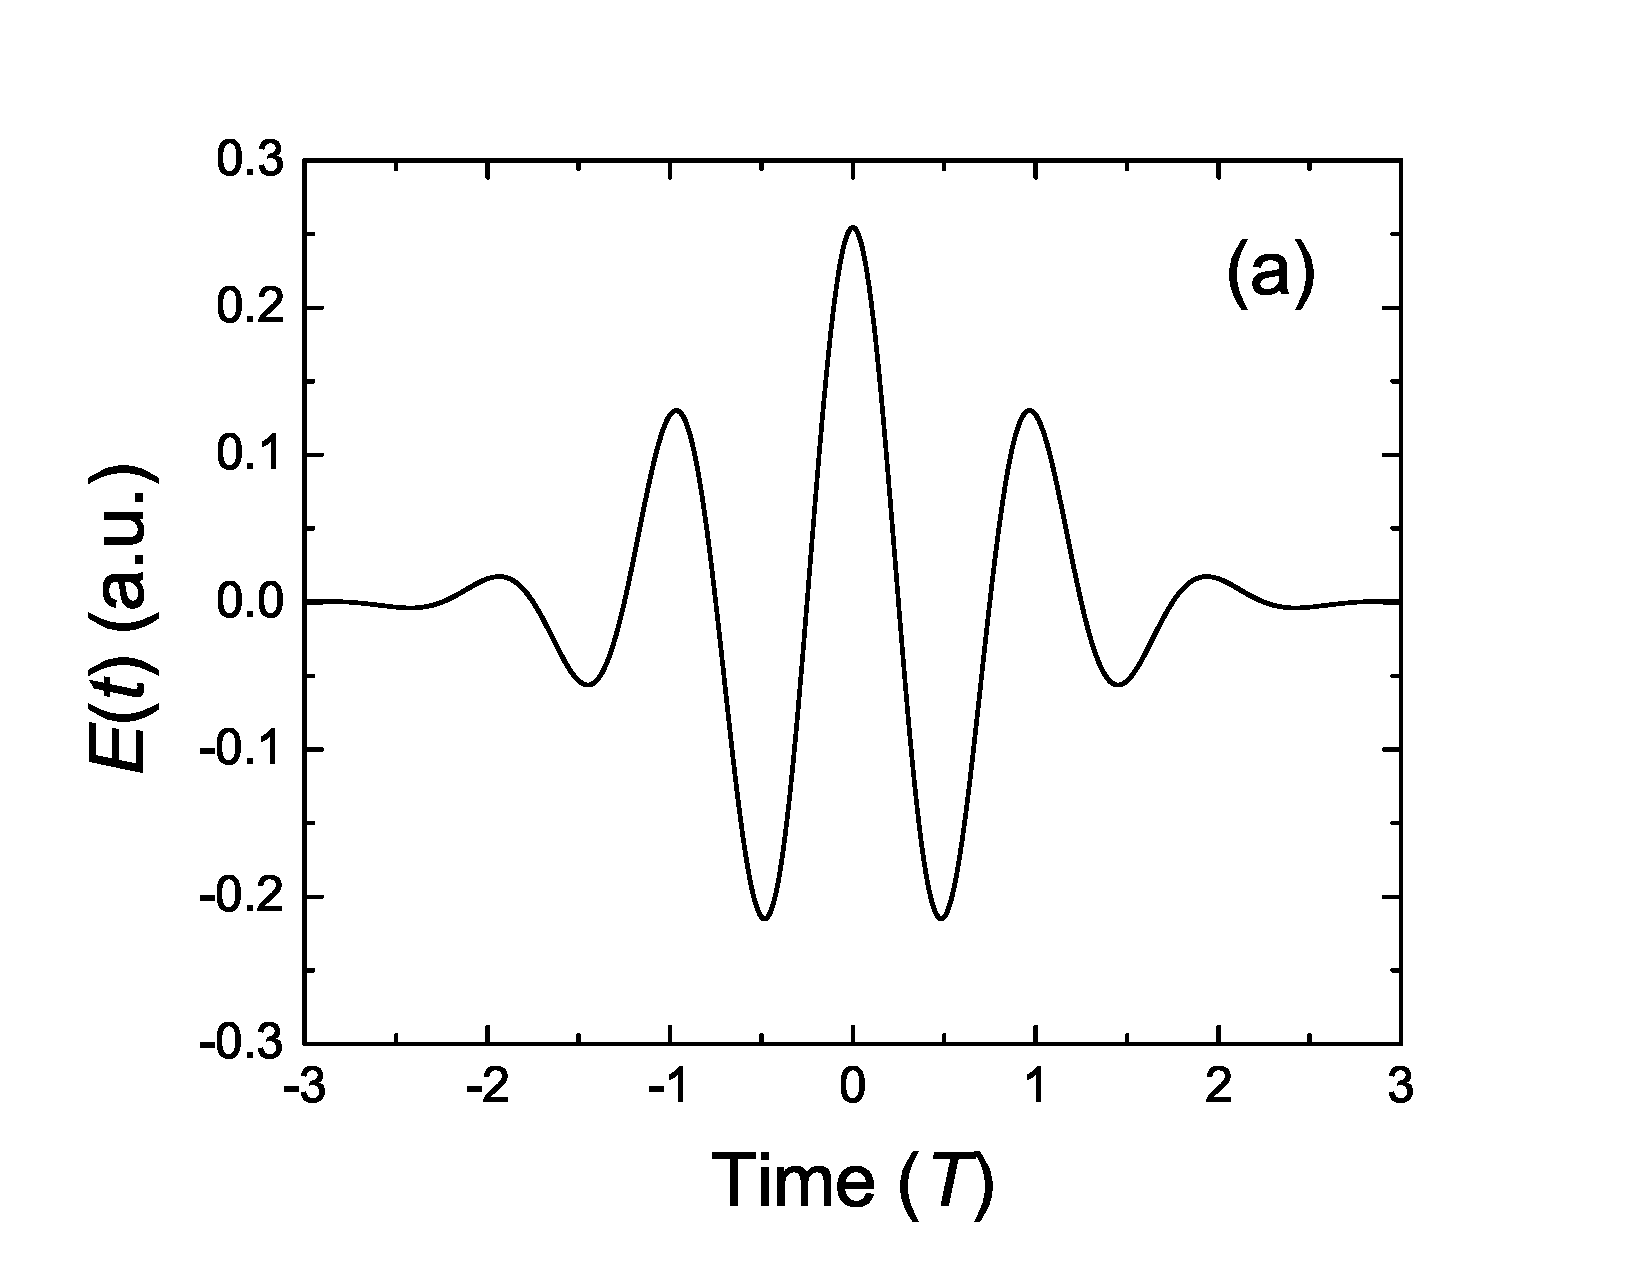
\includegraphics[width=0.4\textwidth]{fig1a.eps}
	}
	\subfigure{
		\label{fig1b}
		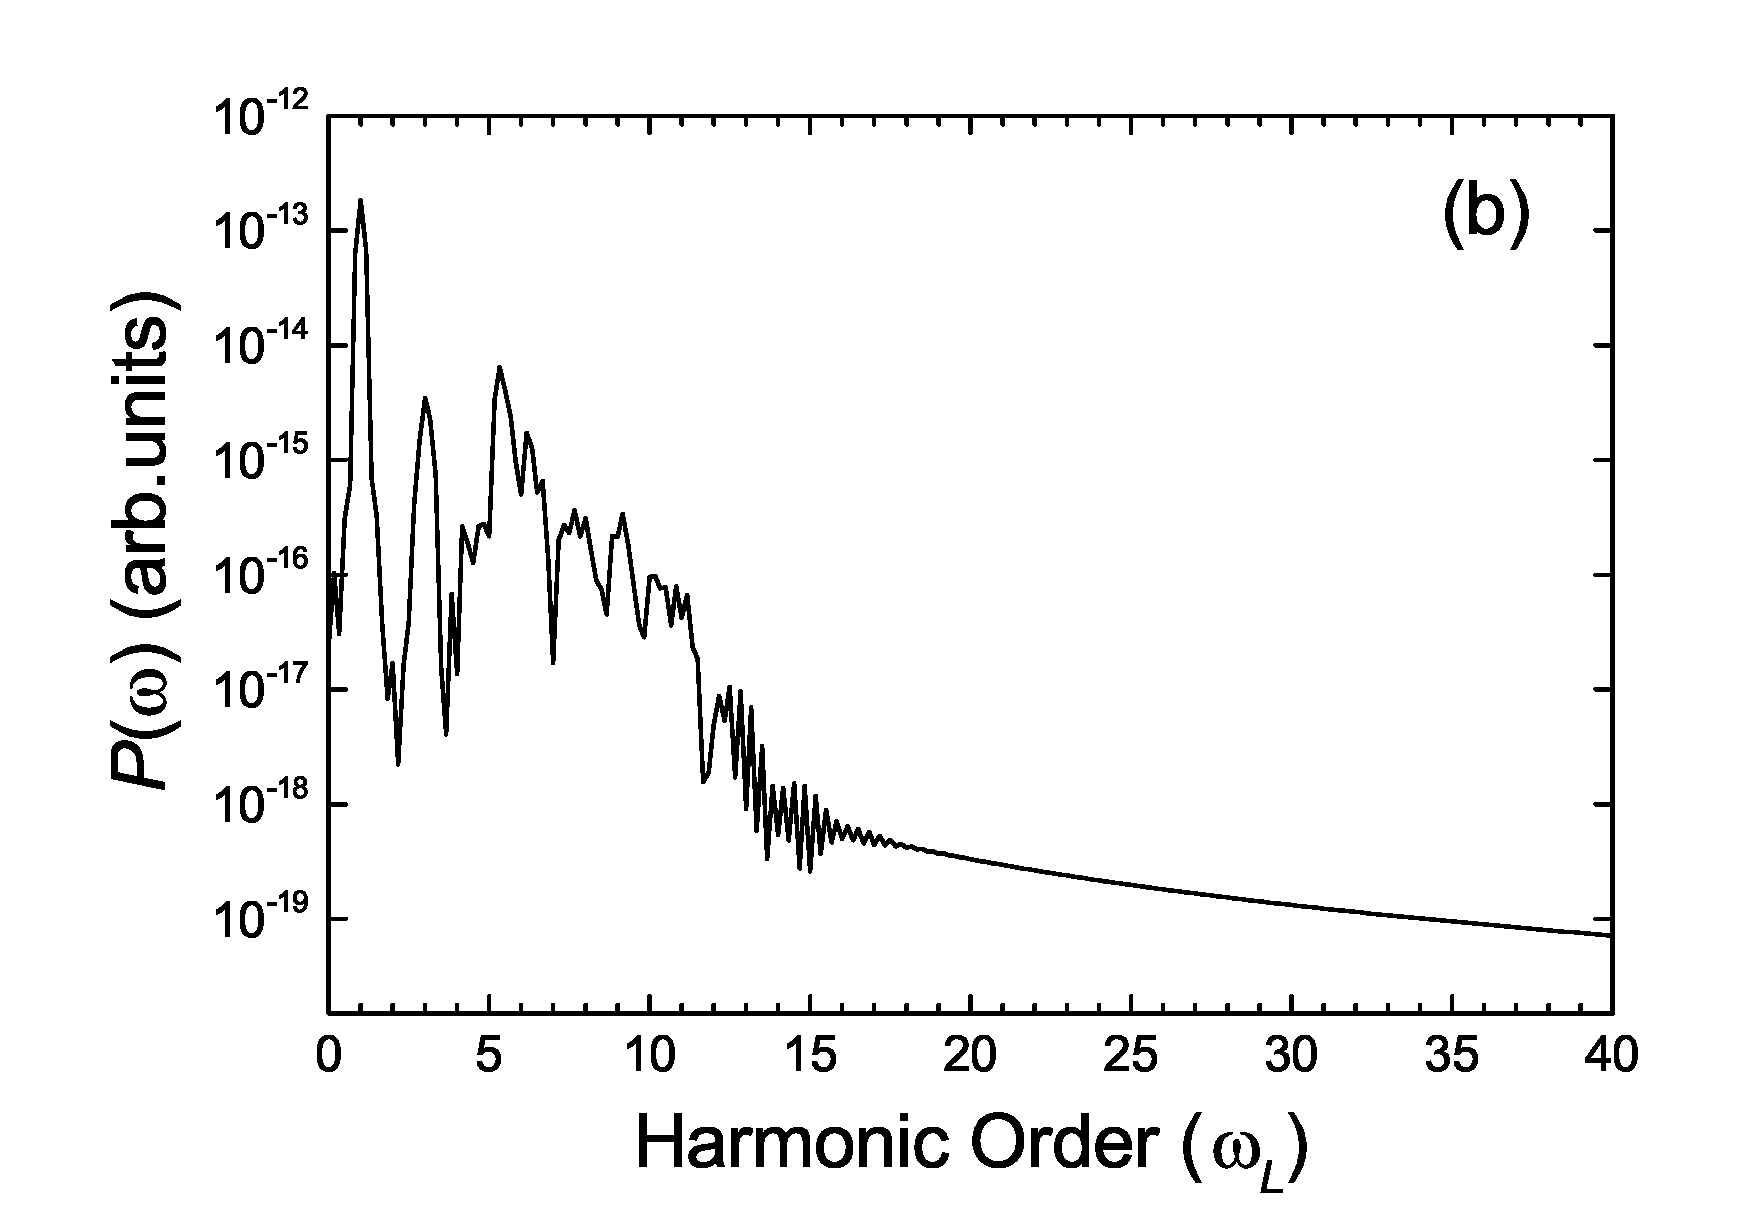
\includegraphics[width=0.4\textwidth]{fig1b.eps}
	}
	\caption{(a) Gaussian laser pulse field without chirp, and (b) the harmonic spectrum driven by this laser pulse. $T$ is the laser period.}
	\label{fig1}
\end{figure}

As expected, the harmonic spectrum shows a generic plateau and cutoff, which can be understood from the picture of the two-level model (new \emph{three-step} method). The harmonic frequency is determined by the transient transition separation between the dressed two adiabatic states

\begin{equation}
\omega  = N{\omega _L} = {\varepsilon _ + } - {\varepsilon _ - } = \sqrt {\omega _0^2 + {{\left[ {2\Omega \left( t \right)} \right]}^2}} .
\label{eq16}
\end{equation}
The separation between the two adiabatic states varies over time, and has a maximum of 

\begin{equation}
{N_{max }}{\omega _L} = \sqrt {\omega _0^2 + {{\left[ {2{\Omega _0}} \right]}^2}} ,
\label{eq17}
\end{equation}
where $ N_{\rm{max}} $ denotes the highest order of the harmonic. From Fig. \ref{fig1b}, it is shown that the cutoff energy from the numerical result is about $ \omega_{\rm{M}}=11\omega_{\rm{L}} $ , which is content with the result from Eq. \ref{eq17}.

Next, we will give a research about the system with permanent dipole moments, while the laser pulse parameters are the same with those in Fig. \ref{fig1a}. The permanent dipole moment parameter is chosen as $ \xi=4 $, and the corresponding harmonic spectrum is shown in Fig. \ref{fig2a}. For this kind of system, the highest order of the harmonic can be theoretically calculated by

\begin{equation}
N_{max }^{'} = {{\sqrt {{{\left[ {{\omega _0} + 2\xi {\Omega _0}} \right]}^2} + {{\left[ {2{\Omega _0}} \right]}^2}} } \mathord{\left/
		{\vphantom {{\sqrt {{{\left[ {{\omega _0} + 2\xi {\Omega _0}} \right]}^2} + {{\left[ {2{\Omega _0}} \right]}^2}} } {{\omega _L}}}} \right.
		\kern-\nulldelimiterspace} {{\omega _L}}}.
\label{eq18}
\end{equation}
It shows that, due to the presence of the permanent dipole moments, the maximum difference of the field-dressed energies is increased compared with the case of without permanent dipole moments (see Eq. \ref{eq17}).Therefore, the harmonic plateau can be extended dramatically even if the Rabi frequency is not increased. According to Eq. \ref{eq18}, $ N_{\rm{max}}^{'}$ equals to 49, which is well accord with the numerical results shown in Fig. \ref{fig2}. If the permanent dipole moment parameter is chosen to be large enough (for example $ \xi=8 $ ), the harmonics of X-ray range will be obtained. However, it can be seen from Fig. \ref{fig2b} that, besides the central peak around cutoff region, the HHG spectra exhibit several well-formed individual peak structures in the plateau region, which decreases the coherence of the HHG and hence is not conducive to the IAP generation. In the following of this paper, the Gaussian pulse with a nonlinear chirped frequency is used to enhance the coherence of the HHG spectrum, and an attosecond pulse train with only two individual peaks can be synthesized with harmonics in the plateau region. 

\begin{figure}[!htbp]
	\centering
	\subfigure{
		\label{fig2a}
		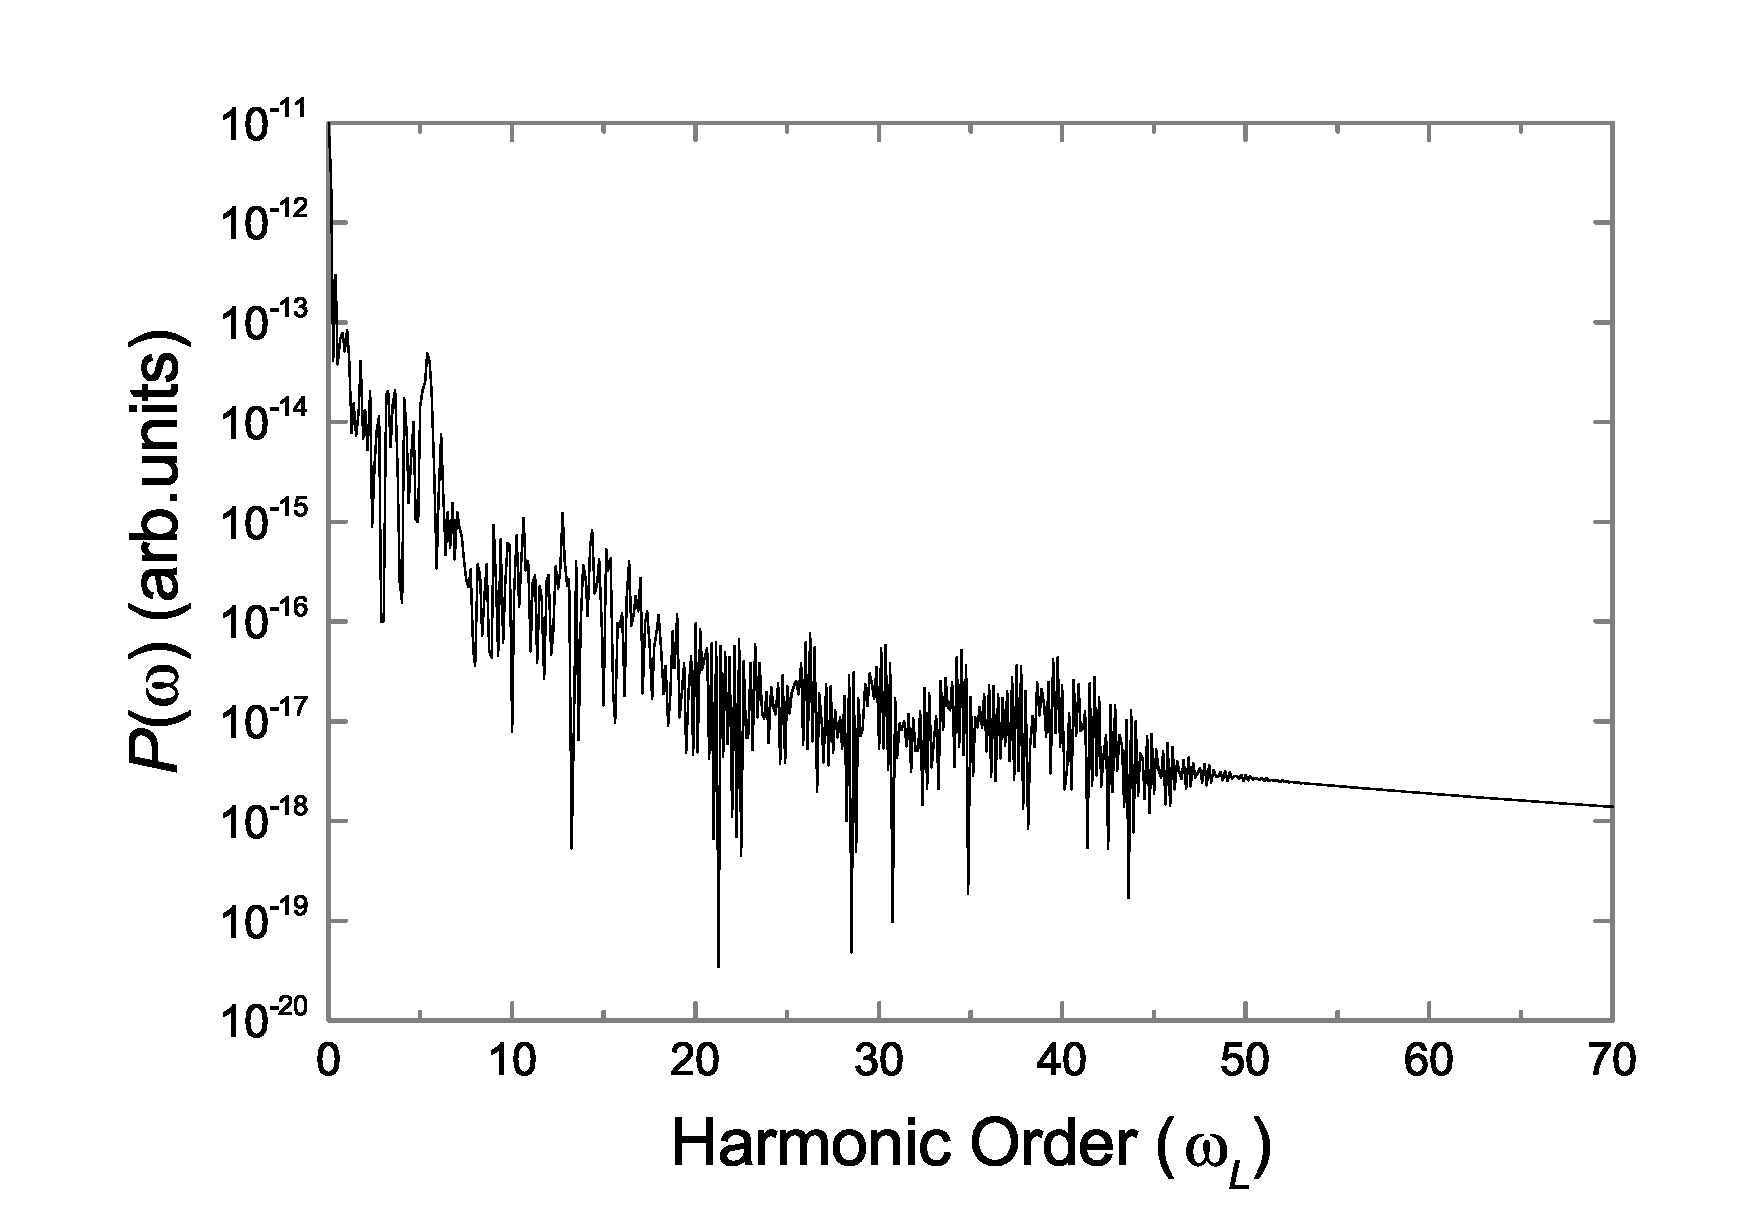
\includegraphics[width=0.45\textwidth,height=0.3\textwidth]{fig2a.eps}
	}
	\hspace{-0.2in}
	\subfigure{
		\label{fig2b}
		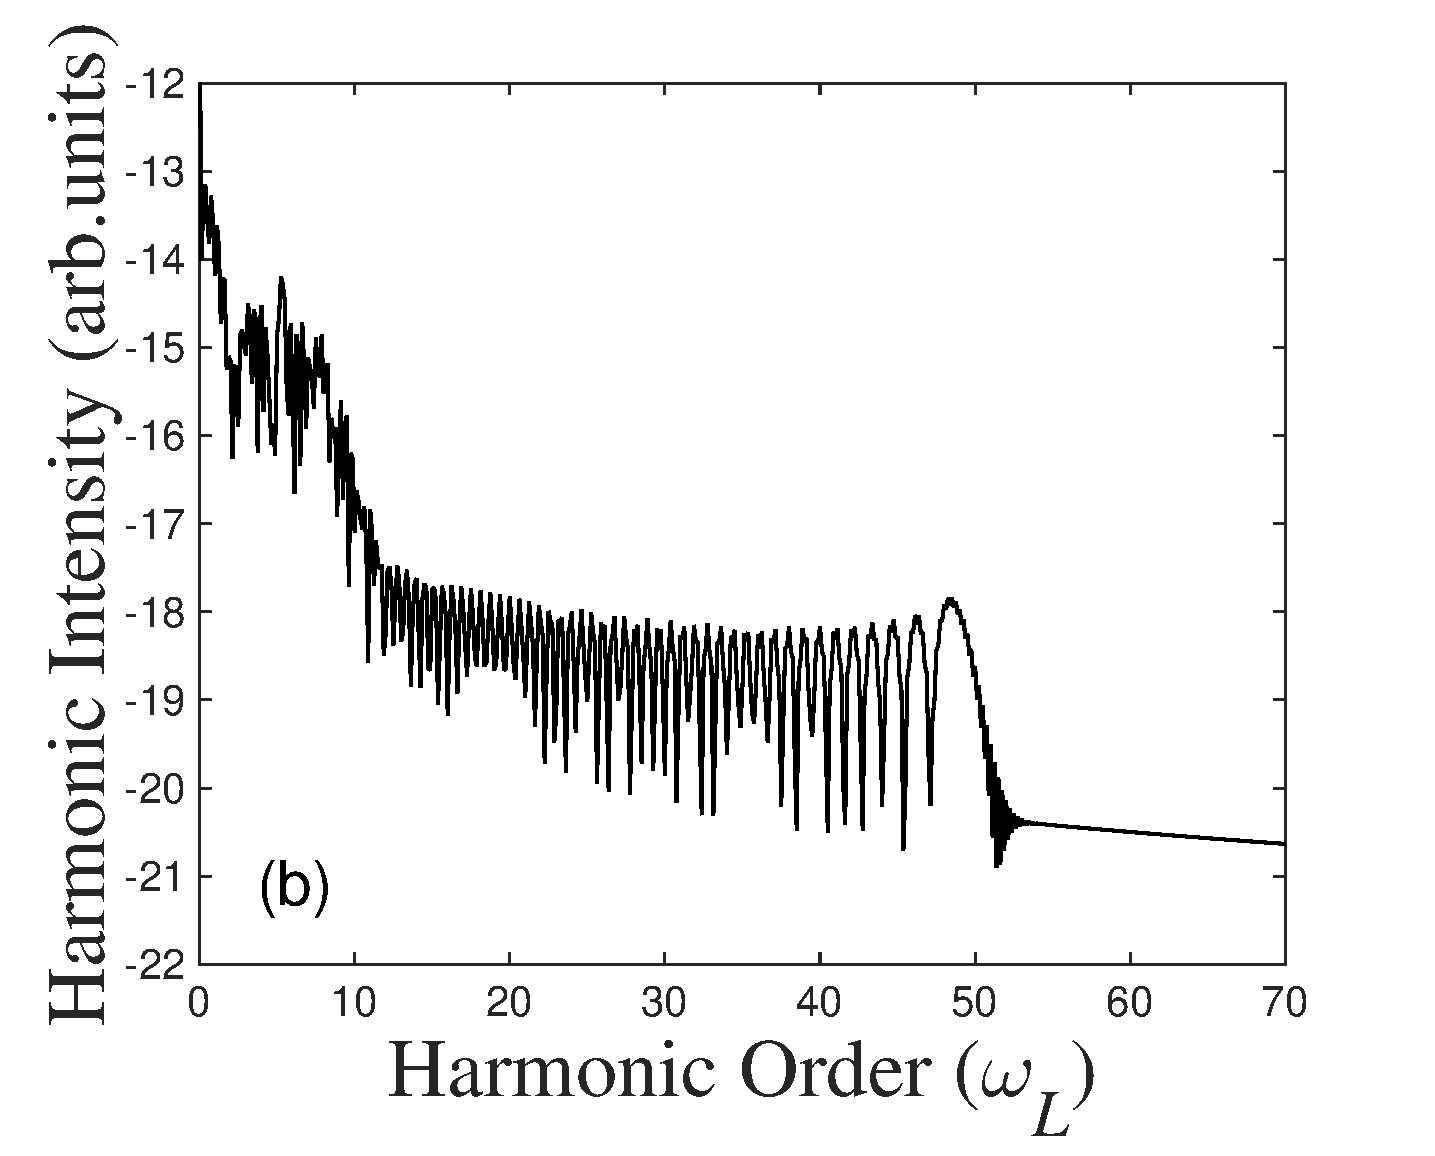
\includegraphics[width=0.5\textwidth,height=0.31\textwidth]{fig2b.eps}
	}
	\caption{(a) The harmonic spectrum of system with permanent dipole moments $ \xi=4 $ driven by the laser pulse without chirp and (b) the corresponding wavelet time-frequency profile. The laser parameters are the same with those in Fig. \ref{fig1a}.}
	\label{fig2}
\end{figure}

A chirp of hyperbolic tangent form is used in the pulse \cite{Carrera-Chirp-PRA-2007}, thus the time profile of carrier envelope phase $ \varphi(t) $  can be given as

\begin{equation}
\varphi \left( t \right) =  - \eta \tanh \left[ {{{\left( {t - {t_d}} \right)} \mathord{\left/
			{\vphantom {{\left( {t - {t_d}} \right)} {{\tau _c}}}} \right.
			\kern-\nulldelimiterspace} {{\tau _c}}}} \right],
\label{eq19}
\end{equation}
where $ \eta $  denotes the frequency sweeping range and $ \tau_{\rm{c}} $ denotes the steepness of the chirp function. $ t_{\rm{d}} $ is set at the middle of the sweep in this paper. If $ \eta=0 $ , the time-dependent carrier envelope phase $ \varphi(t) $  will equals to be zero, the pulse is chirp free then.

\begin{figure}[!htbp]
	\centering
	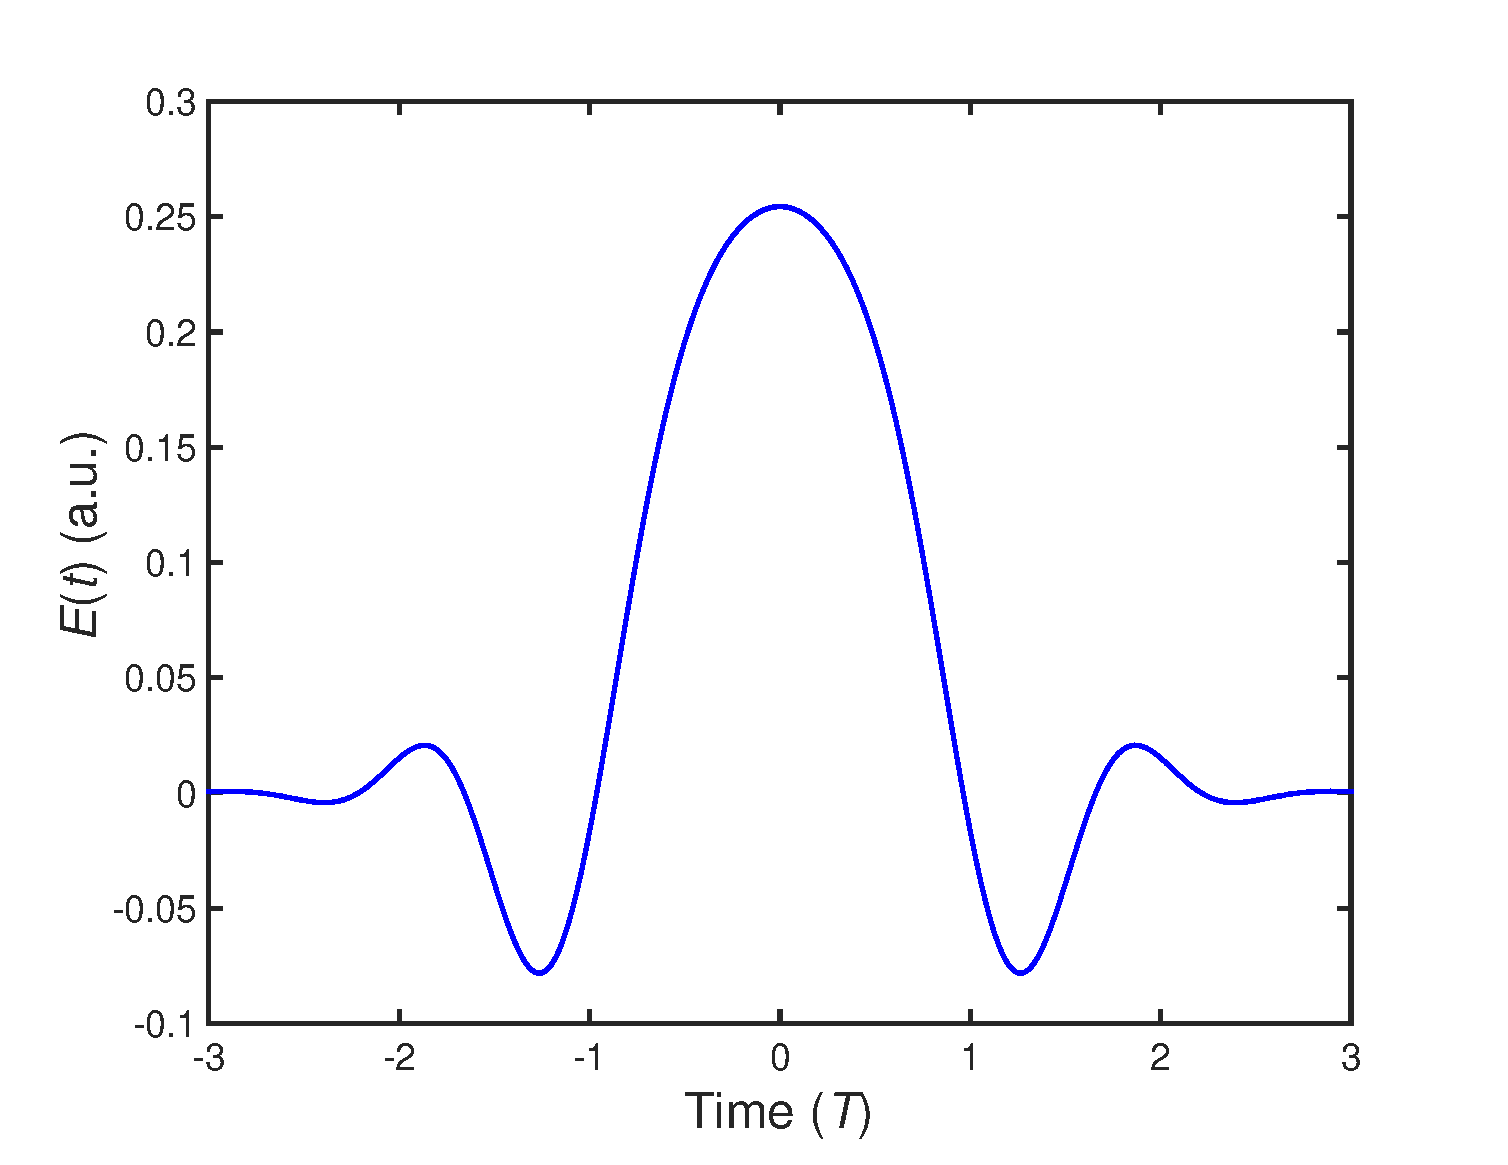
\includegraphics[width=0.45\textwidth]{fig3}
	\caption{The laser pulse with chirped frequency. $ \eta=6.25 $, $ \tau_{\rm{c}}=120 $, the other laser parameters are the same with those in Fig. \ref{fig1a}.}
	\label{fig3}
\end{figure}

As we know that, the chirp frequency has a large influence on the pulse carriers. Fig. \ref{fig3} shows the laser pulse with the chirp parameters $ \eta=6.25 $ and $ \tau_{\rm{c}}=120$. The oscillatory periodicity and the up-down symmetry of the laser pulse is changed, as a result, the center carrier gets broader, the side carriers get weaker while the pulse peak remains invariant. According to the level crossing theory, the time-frequency spectrum shares the same shape with the positive branch of the pulse amplitude \cite{WANG-ZHONG-YANG-Two-Level-Attosecond-generation-1999}. If the value difference between the pulse center peak and the second peak gets larger, there will be more harmonics emit with as many as two trajectories. These harmonics obviously have better coherence than those emit with more than two trajectories. However, the coherence is somehow weakened for the increase of the time interval between the two trajectories which originate from the getting broader of the center carrier. Since it is contradictory for the center carrier to get narrower and for the side carriers to get weaker, we chose a balanced chirp parameters as  $ \eta=6.25 $ and $ \tau_{\rm{c}}=120 $ , which makes the side carriers quite weak and the center carrier not too broad. 

\begin{figure}[!htbp]
	\centering
	\subfigure{
		\label{fig4a}
		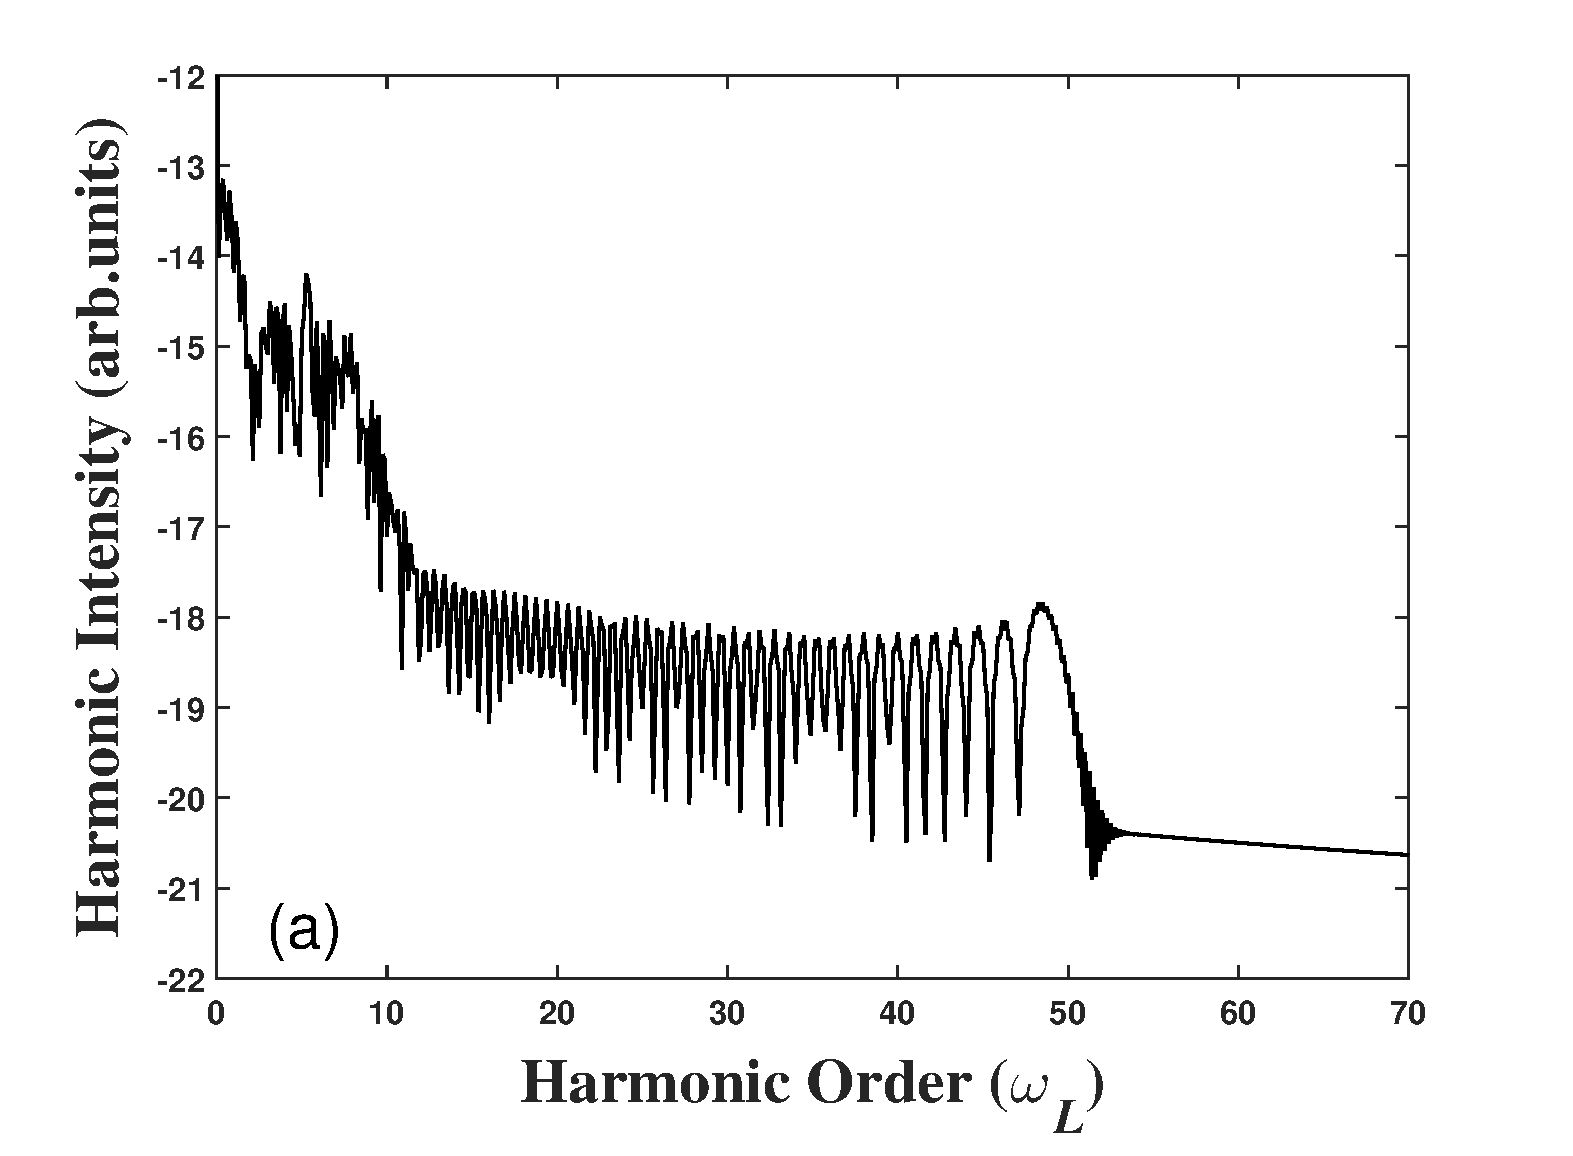
\includegraphics[width=0.4\textwidth]{fig4a.eps}
	}
	\subfigure{
		\label{fig4b}
		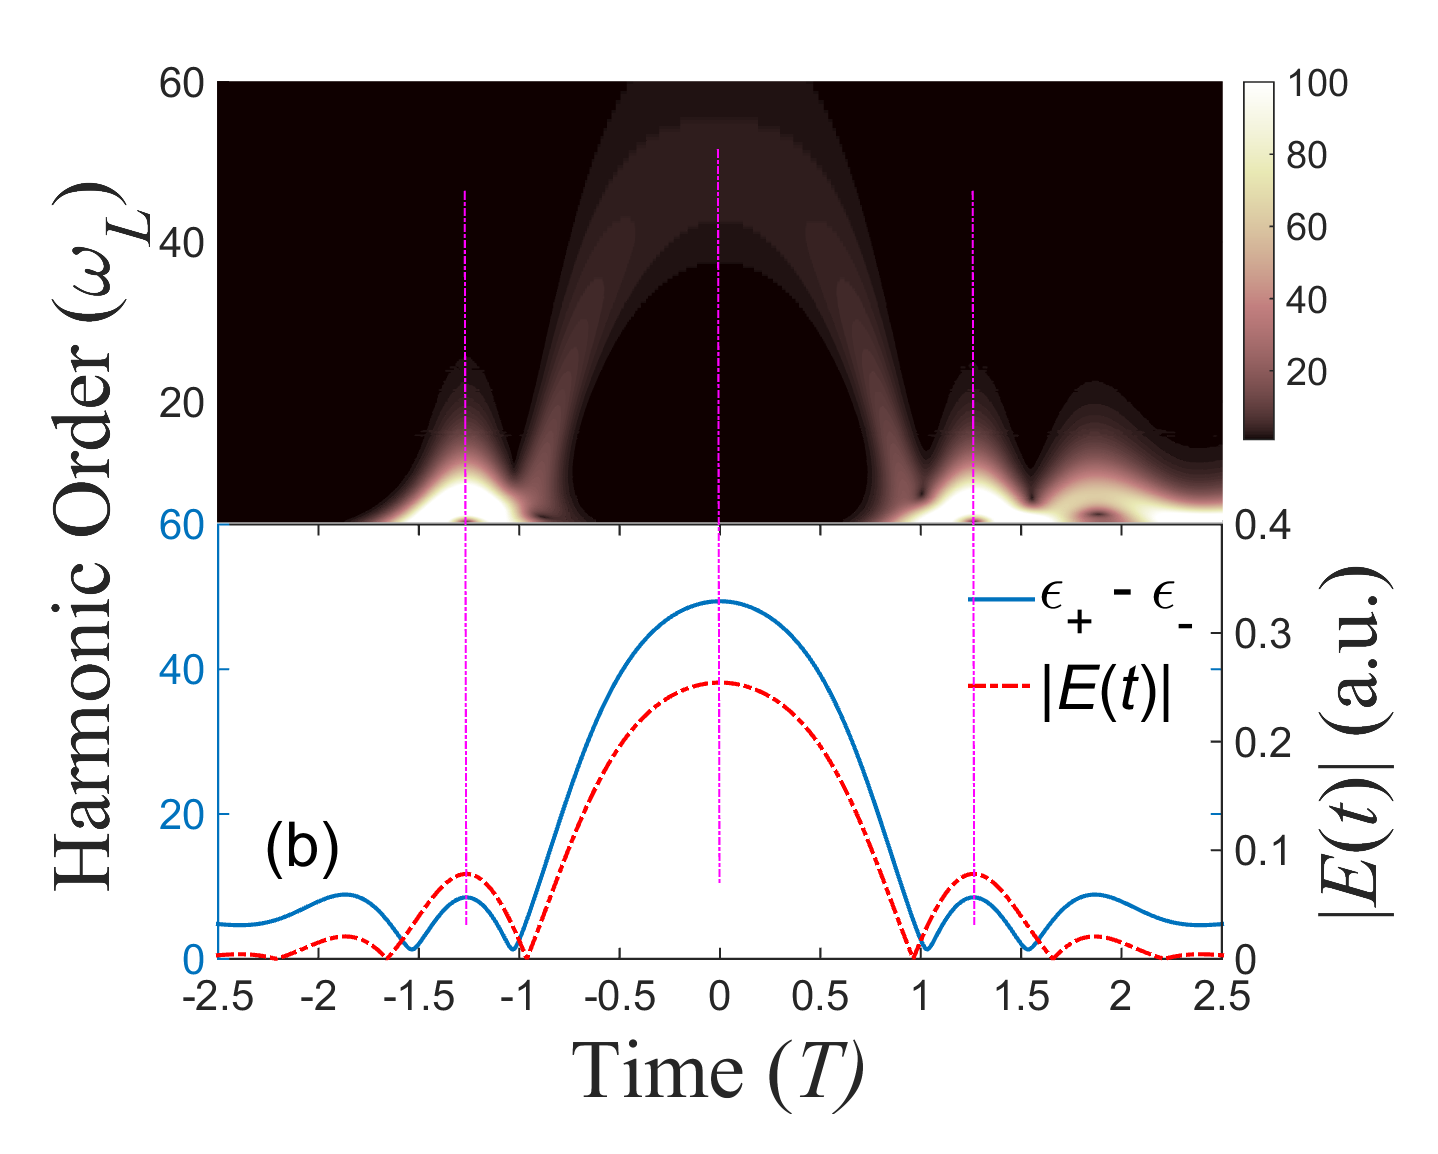
\includegraphics[width=0.4\textwidth]{fig4b.eps}
	}
	\caption{(a) The HHG spectrum of system with permanent dipole moments ($ \xi=4 $) driven by the laser pulse with chirped frequency, and (b) the corresponding wavelet time-frequency profile.}
	\label{fig4}
\end{figure}

Fig. \ref{fig4}(a) shows the harmonic spectrum of the system with permanent dipole moments ($ \xi=4 $) driven by the chirped laser pulse. The time-frequency profile of the harmonic spectrum corresponding to Fig. \ref{fig4a} is shown in Fig. \ref{fig4b}. Since the pulse envelope is invariant to the chirped frequency ($ E_{0} $ and $ \Omega_{0} $ are not changed), according to Eq. (\ref{eq18}), the harmonic spectra should have the same cutoff energy as the cases in Fig. \ref{fig2}. This is confirmed by the numerical results from Fig. \ref{fig4}. However, there are only two well-formed individual peak structures besides the central peak in the time-frequency spectrum while the case of without chirp has four. Moreover, the value difference between the central peak and the second peak is much larger than the corresponding one shown in Fig. \ref{fig2b}. Therefore, there are much more harmonics that have two trajectories at most with the plateau region, as a result, the coherence of the harmonic spectrum is enhanced. As it is shown in Fig. \ref{fig4a} that, the harmonic spectrum have a large plateau region that is much smoother than the corresponding one shown in Fig. \ref{fig2a}. 

Next we select the harmonics within the plateau to synthesize attosecond pulses. For the system with the permanent dipole moments ($ \xi=4 $), we chose all the harmonics (including the even orders) from the $ 25\rm{th} $ to $ 40\rm{th} $ for the spectrum driven by the chirped laser pulse, while chose all the odd harmonics in the same region for the spectrum driven by the non-chirped laser pulse. The results are shown in Fig. \ref{fig5}. There is an attosecond pulse train generated with six individual peaks for the case driven by the non-chirped laser pulse, while there is also an attosecond pulse train generated which has only two individual peaks. Although there is no IAP generated, it shows a big progress in the enhancement of the coherence of the harmonic spectrum. 

\begin{figure}[!htbp]
	\centering
	\subfigure{
		\label{fig5a}
		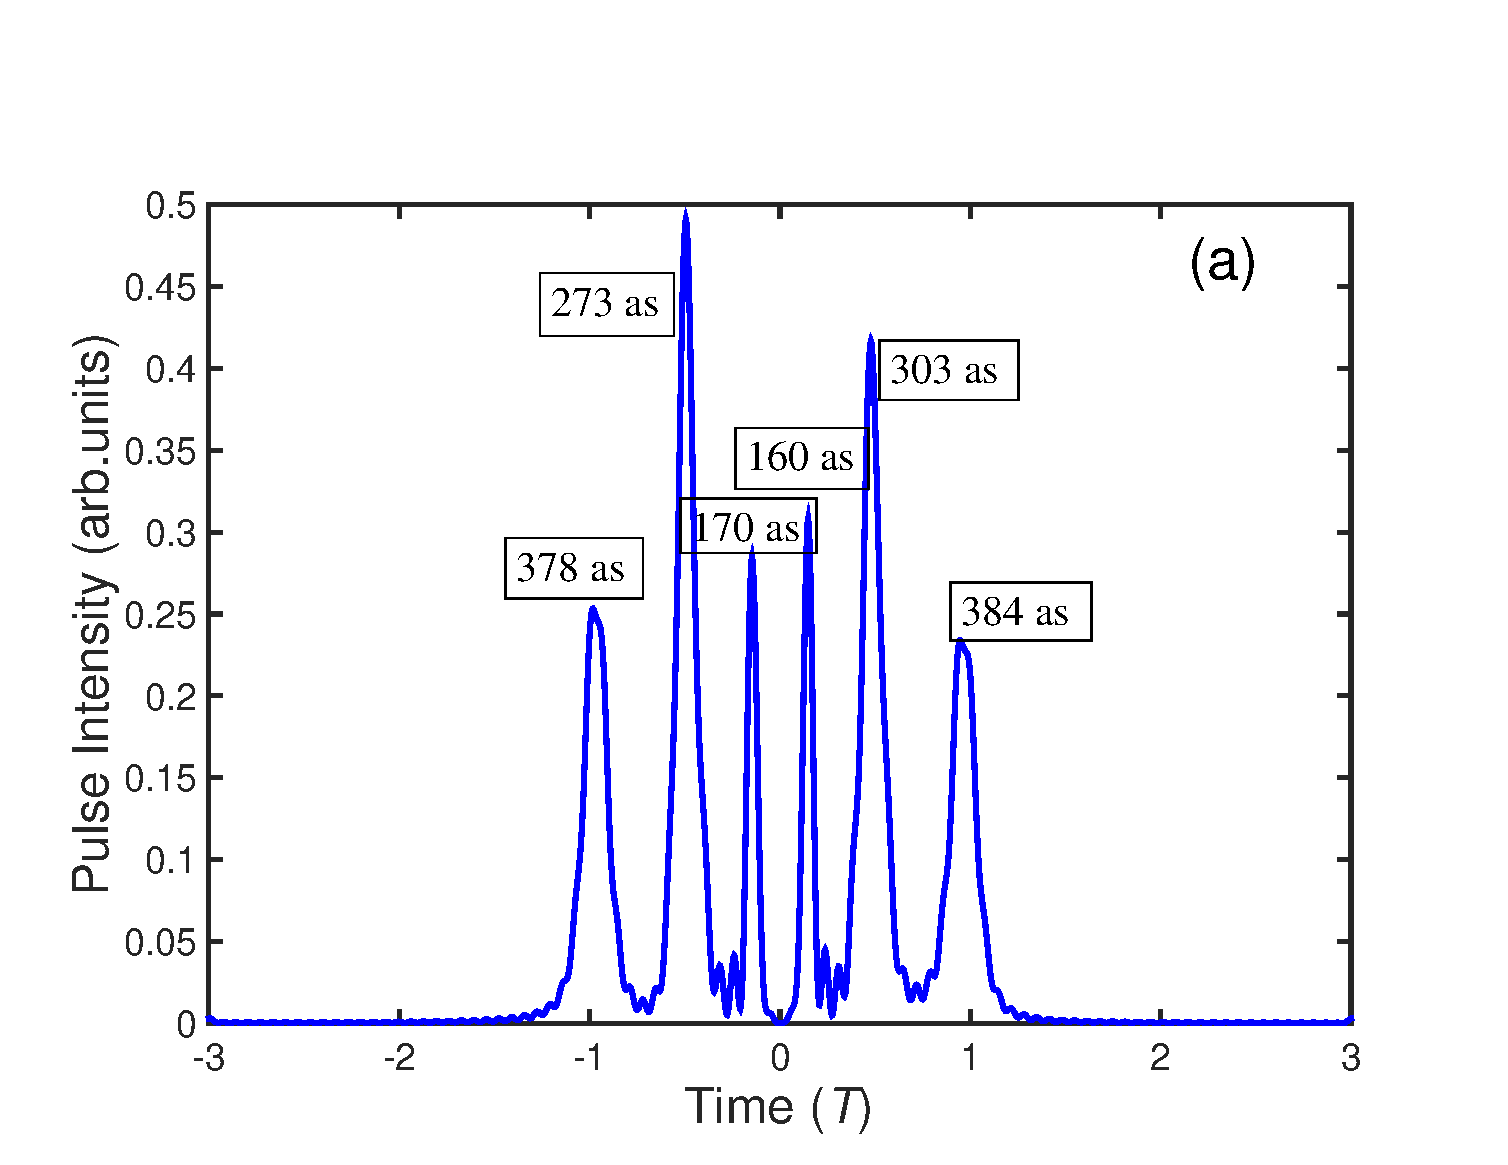
\includegraphics[width=0.4\textwidth]{fig5a.eps}
	}
%	\hspace{0.1in}
	\subfigure{
		\label{fig5b}
		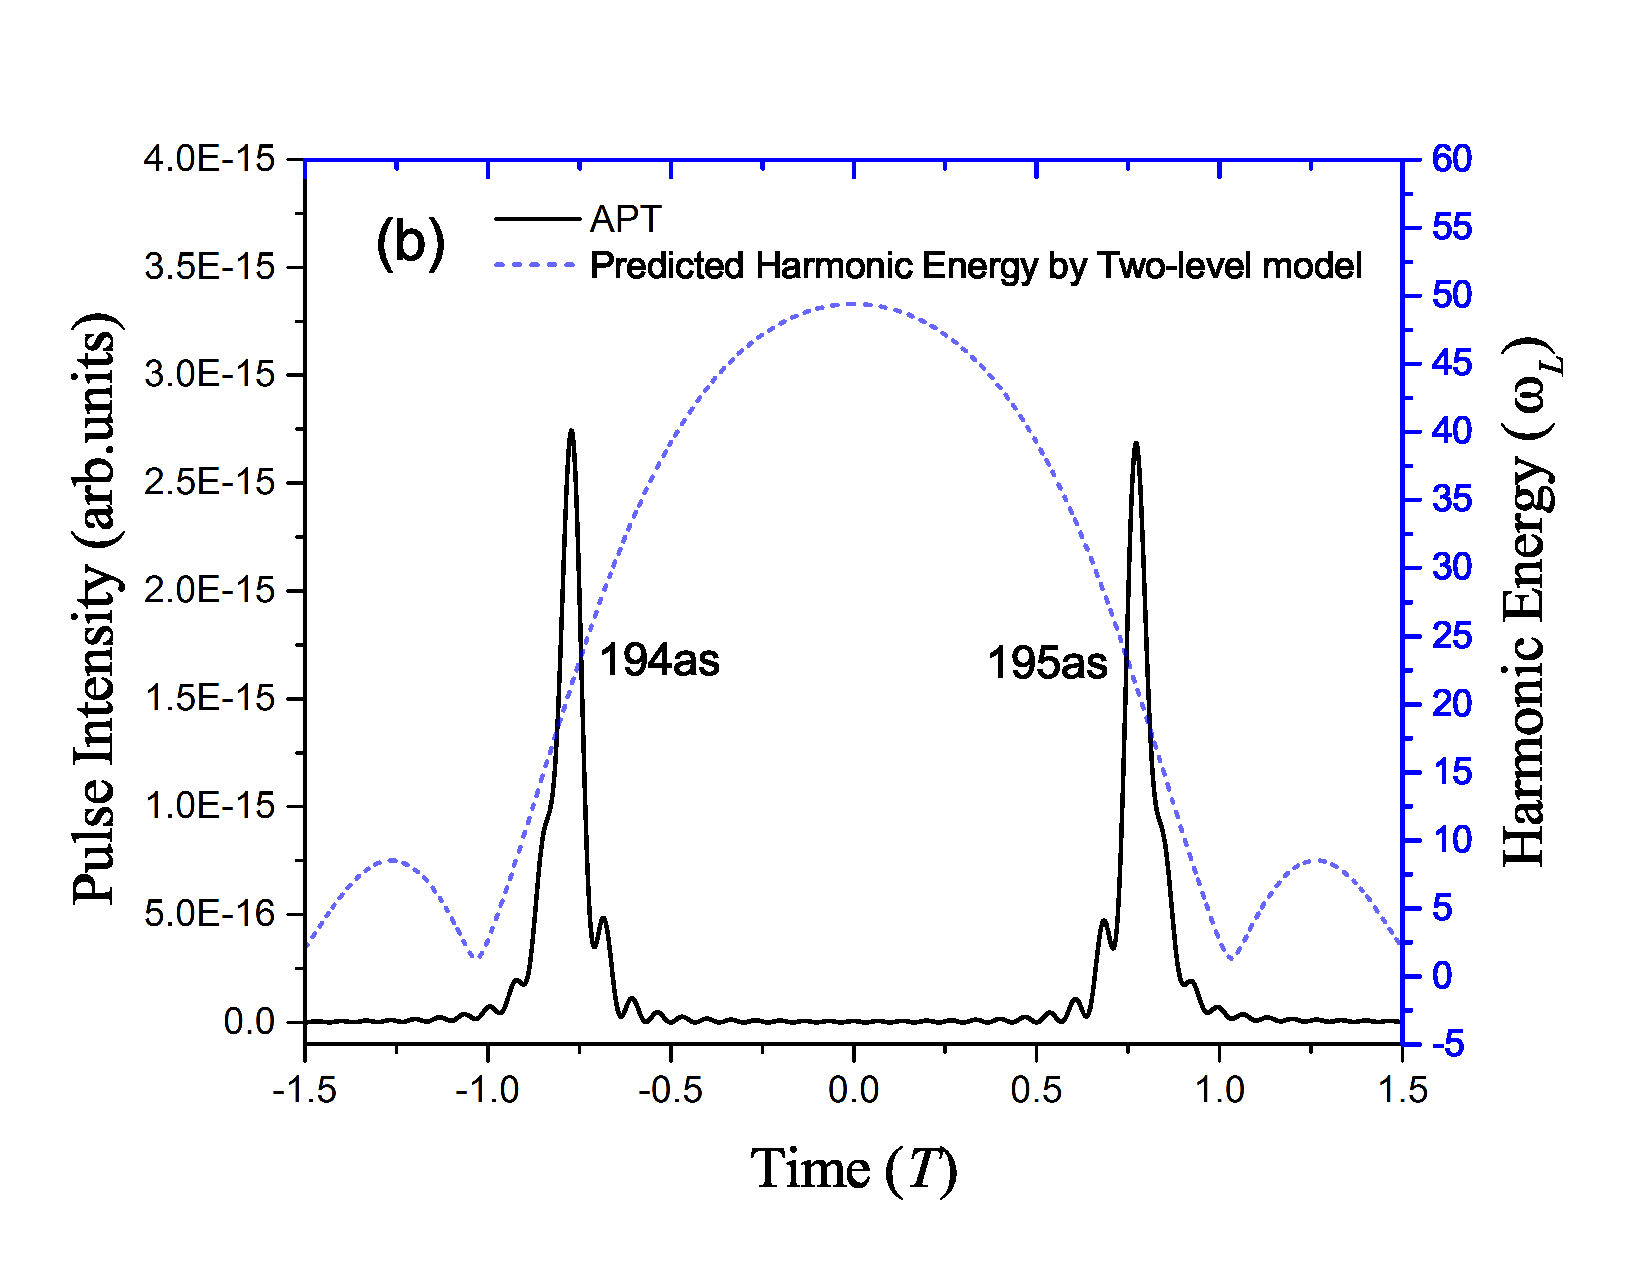
\includegraphics[width=0.4\textwidth]{fig5b.eps}
	}
	\caption{The generated attosecond pulses from the spectra driven by (a) the laser pulse without chirp and (b) with chirp. The system has permanent dipole moments of $ \xi=4 $.}
	\label{fig5}
\end{figure}	

Now we have successfully demonstrated that the combination of the controls of chirped laser pulse and permanent dipole moment can be effective to the attosecond pulse generation. Because of the permanent dipole moment, much more harmonics were used to synthesize attosecond pulse, furthermore the chirped driving laser pulse enhanced the coherence of the harmonics. However, an IAP has not obtained by synthesizing the harmonics within the plateau. As we know, an IAP can be generated by synthesizing the harmonics near the end of the plateau (or cutoff region), but the pulse intensity is very weak. Therefore we will investigate the propagation condition and expect the increase of the harmonic signal intensity. The part medium parameters are: $ \bar{N}=7.5\times10^{24} \textrm{m}^{-3}$, $ T_{1}=1.0\times10^{-12} \textrm{s} $,$ T_{2}=0.5\times10^{-12} \textrm{s} $ \cite{Kalosha-Two-Level-PRL-1999} and the rest medium parameters and all the laser parameters are all the same with the non-propagation cases. For the chirped laser pulse, the initial boundary condition is

\begin{equation}
\begin{array}{l}
{E_x}\left( {z,t = 0} \right) = {E_0}\exp \left[ { - 4\ln 2{{\left( {\frac{{z - {z_0}}}{{c\tau }}} \right)}^2}} \right]\cos \left[ {{\omega _L}{{\left( {z - {z_0}} \right)} \mathord{\left/
			{\vphantom {{\left( {z - {z_0}} \right)} c}} \right.
			\kern-\nulldelimiterspace} c} + \eta \tanh \frac{{z - {z_0}}}{{c{\tau _c}}}} \right],\\
{H_y}\left( {z,t = 0} \right) = \sqrt {{{{\varepsilon _0}} \mathord{\left/
			{\vphantom {{{\varepsilon _0}} {{\mu _0}}}} \right.
			\kern-\nulldelimiterspace} {{\mu _0}}}} {E_x}\left( {z,t = 0} \right).
\end{array}
\label{eq20}
\end{equation} 
We consider both the cases of laser pulses with and without chirp, and only the medium with the permanent dipole moments. We choose 9 groups of thickness of the medium from 10 to 90 $ \mu $m evenly divided by 10 $ \mu $m, and study the harmonic generation in the transmission interface, respectively. 

\begin{figure}[!htbp]
\centering
\subfigure{
	\label{fig6a}
	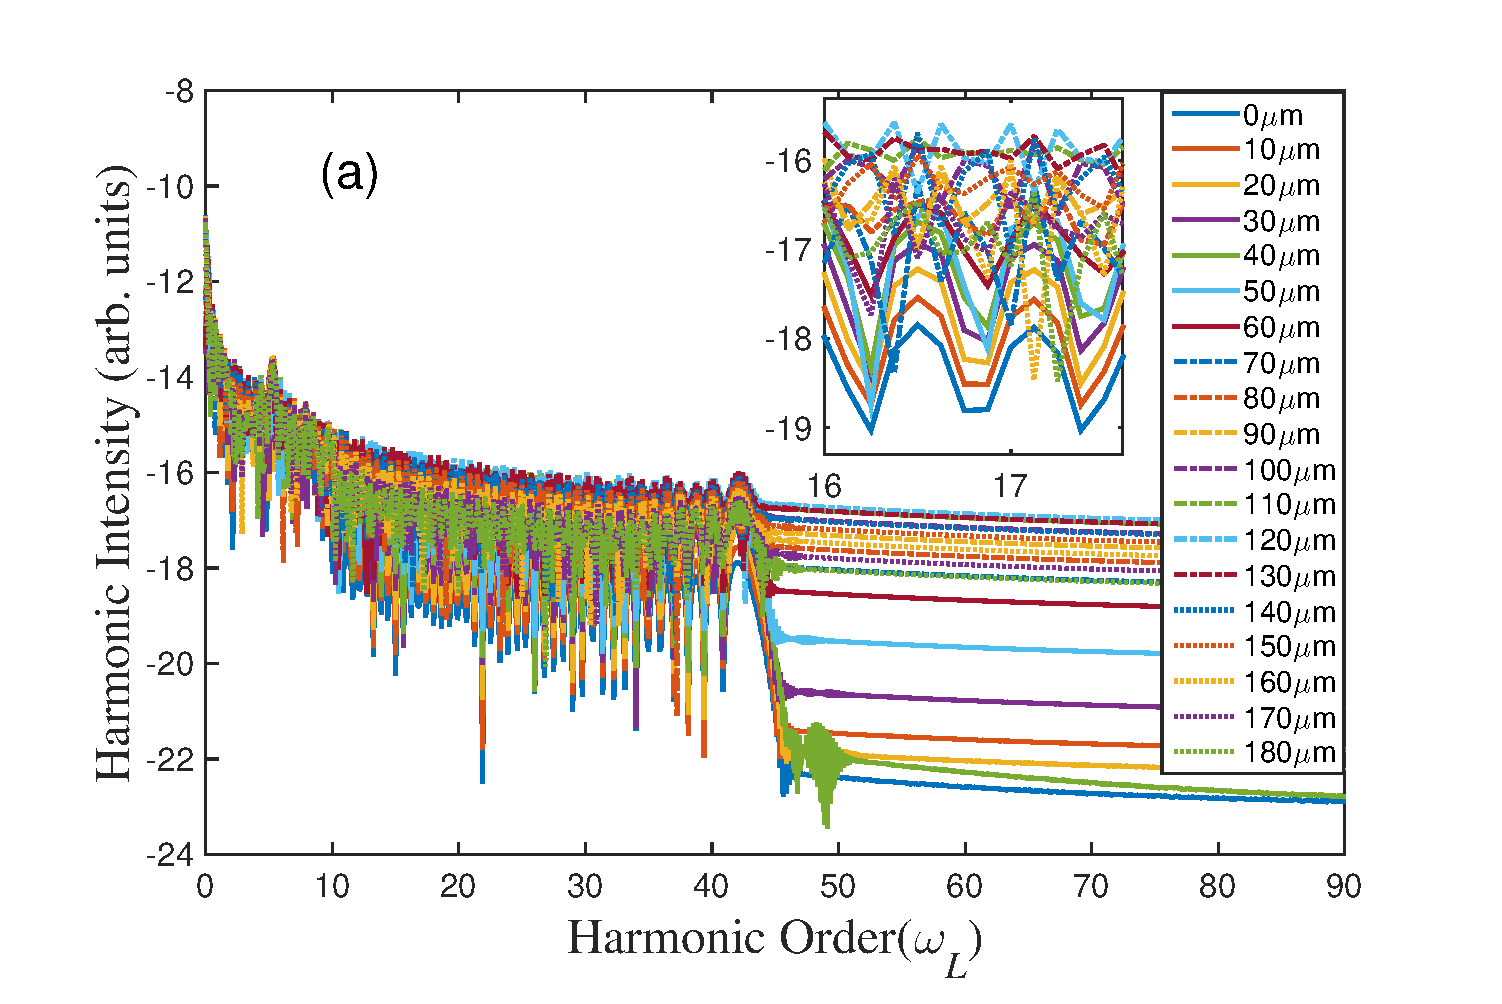
\includegraphics[width=0.4\textwidth]{fig6a.eps}
	}
%\hspace{0.2in}
\subfigure{
	\label{fig6b}
	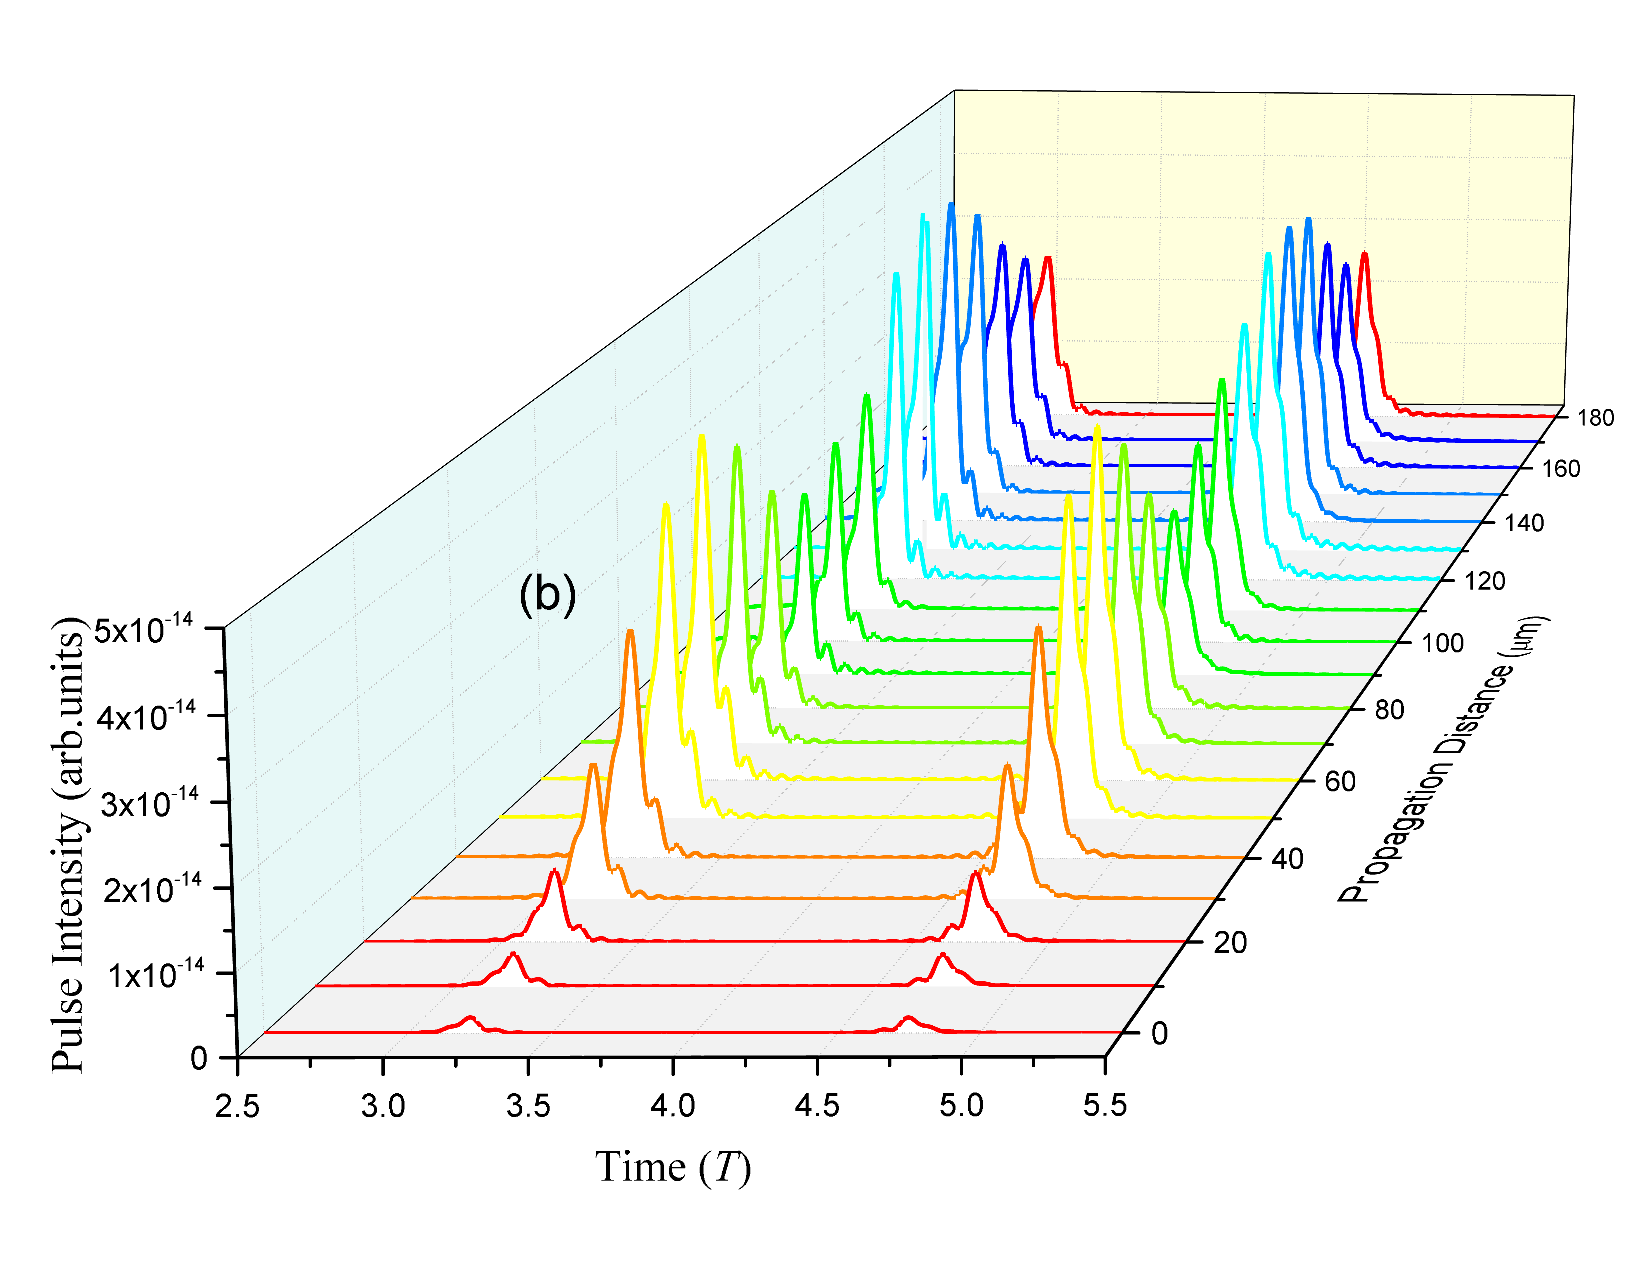
\includegraphics[width=0.4\textwidth]{fig6b.eps}
	}
\caption{The harmonic spectra of system with permanent dipole moments ($ \xi=4 $) driven by the laser pulse (a) without chirp, and (b) with chirp.}
\label{fig6}
\end{figure}

Fig. \ref{fig6} shows the harmonic spectra of system with permanent dipole moments ($ \xi=4 $) driven by the laser pulse with and without chirp for 9 propagation distances. A peak appears in the position of about  $ 5.36\;\omega_{\rm{L}} $ with considerable value. We know that it is the results of the resonant absorption, and this peak also exists in the non-propagation case but it is not so strong. Here we will focus on the cutoff region of the spectrum because we can only synthesize the continuum harmonics within this region to generate an IAP. It shows that, for the both cases, the harmonic intensity varies with different propagation distance. However, this variation is not monotonically increasing or monotonically decreasing. There is a maximum value with the propagation of the laser pulse. We select $37\rm{th}$-$50\rm{th}$ and $41\rm{st}$-$45\rm{th}$ harmonics in the cutoff region for the chirp case and the non-chirp case, respectively, to synthesize an IAP. Fig. \ref{fig7} shows the results and Table \ref{table1} is the corresponding statistics for the generated pulse peak intensity and the FWHM. Even though the selected harmonics are in the cutoff region, the synthesized IAP can be as strong as those pulses synthesized by selecting the plateau harmonics [Fig. \ref{fig5a}] and even stronger than the two generated pulses of the chirp case [Fig. \ref{fig5b}]. However, the pulse intensity cannot progressively increase, it will has a maximum value for an proper propagation distance. And the pulse for the chirp or non-chirp case almost has the same duration for different propagation distance because of the same harmonics selected. We note that, for the modulation of the chirped frequency, the spectral width of the continuum is different for the two cases. We will select harmonics as much as possible to synthesize more intensive IAP. Therefore we selected different orders of harmonic for the two cases, while this cannot influence our demonstration  since only the propagation effect is studied here.
\begin{figure}[!htbp]
	\centering
	\subfigure{
		\label{fig7a}
		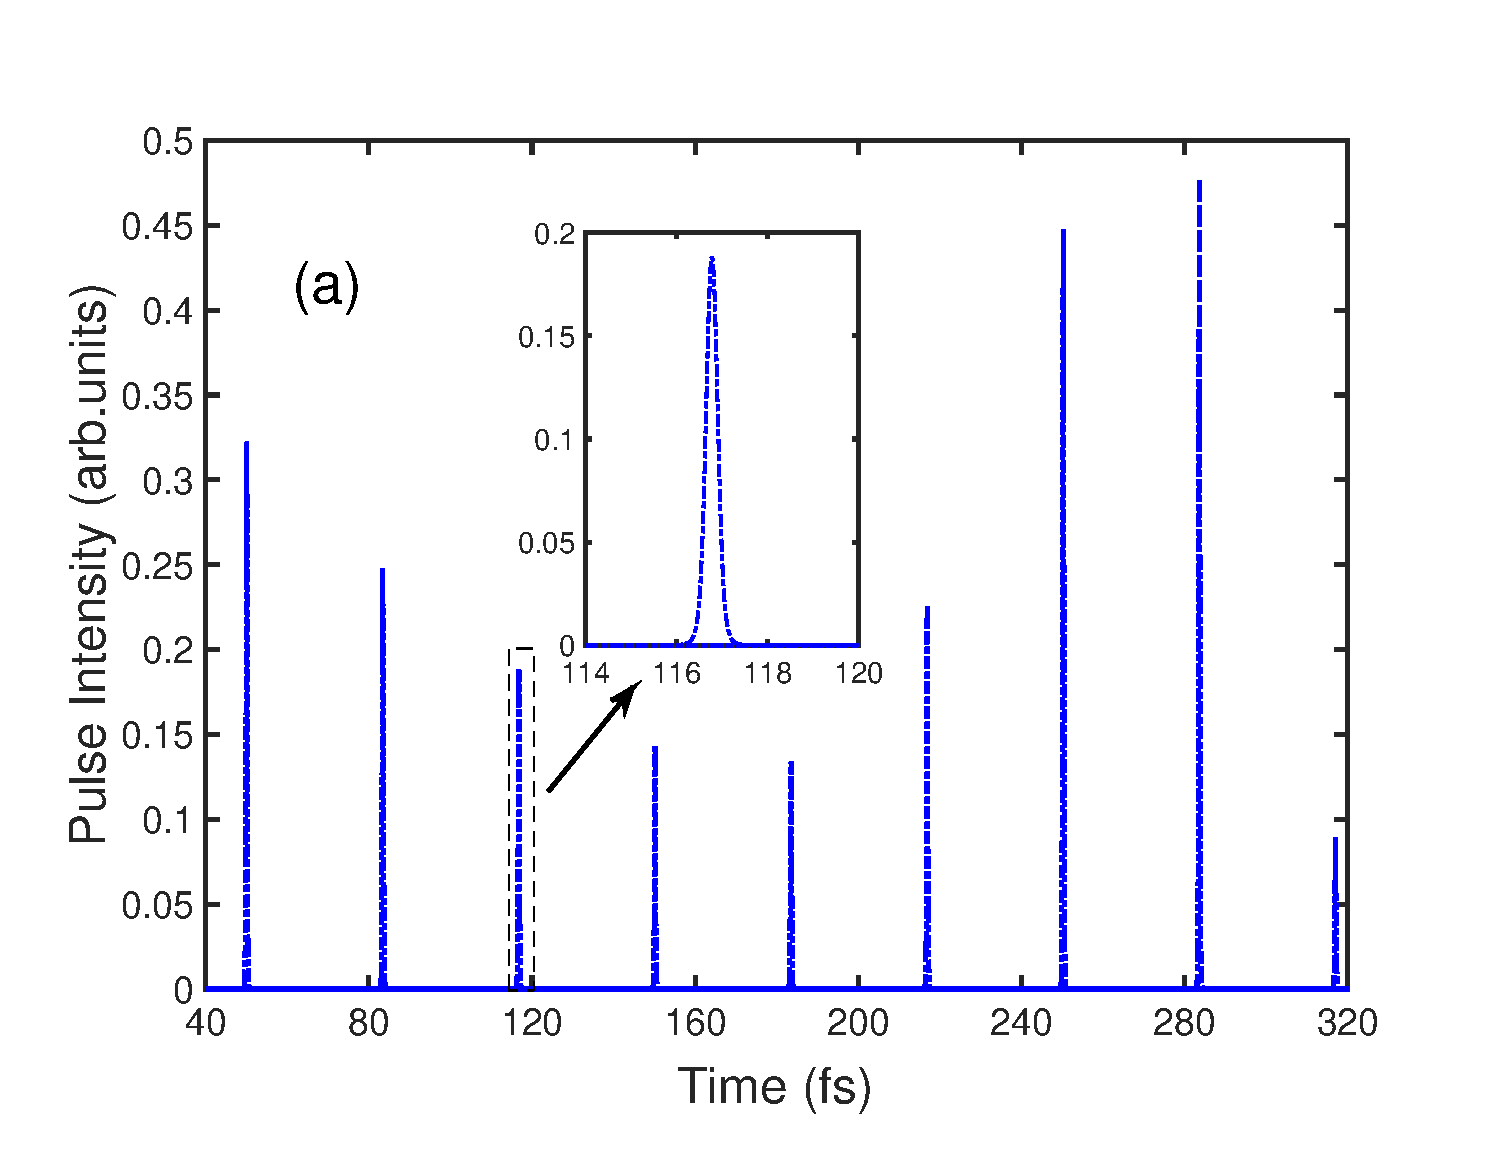
\includegraphics[width=0.4\textwidth]{fig7a.eps}
	}
	\hspace{-0.2in}
	\subfigure{
		\label{fig7b}
		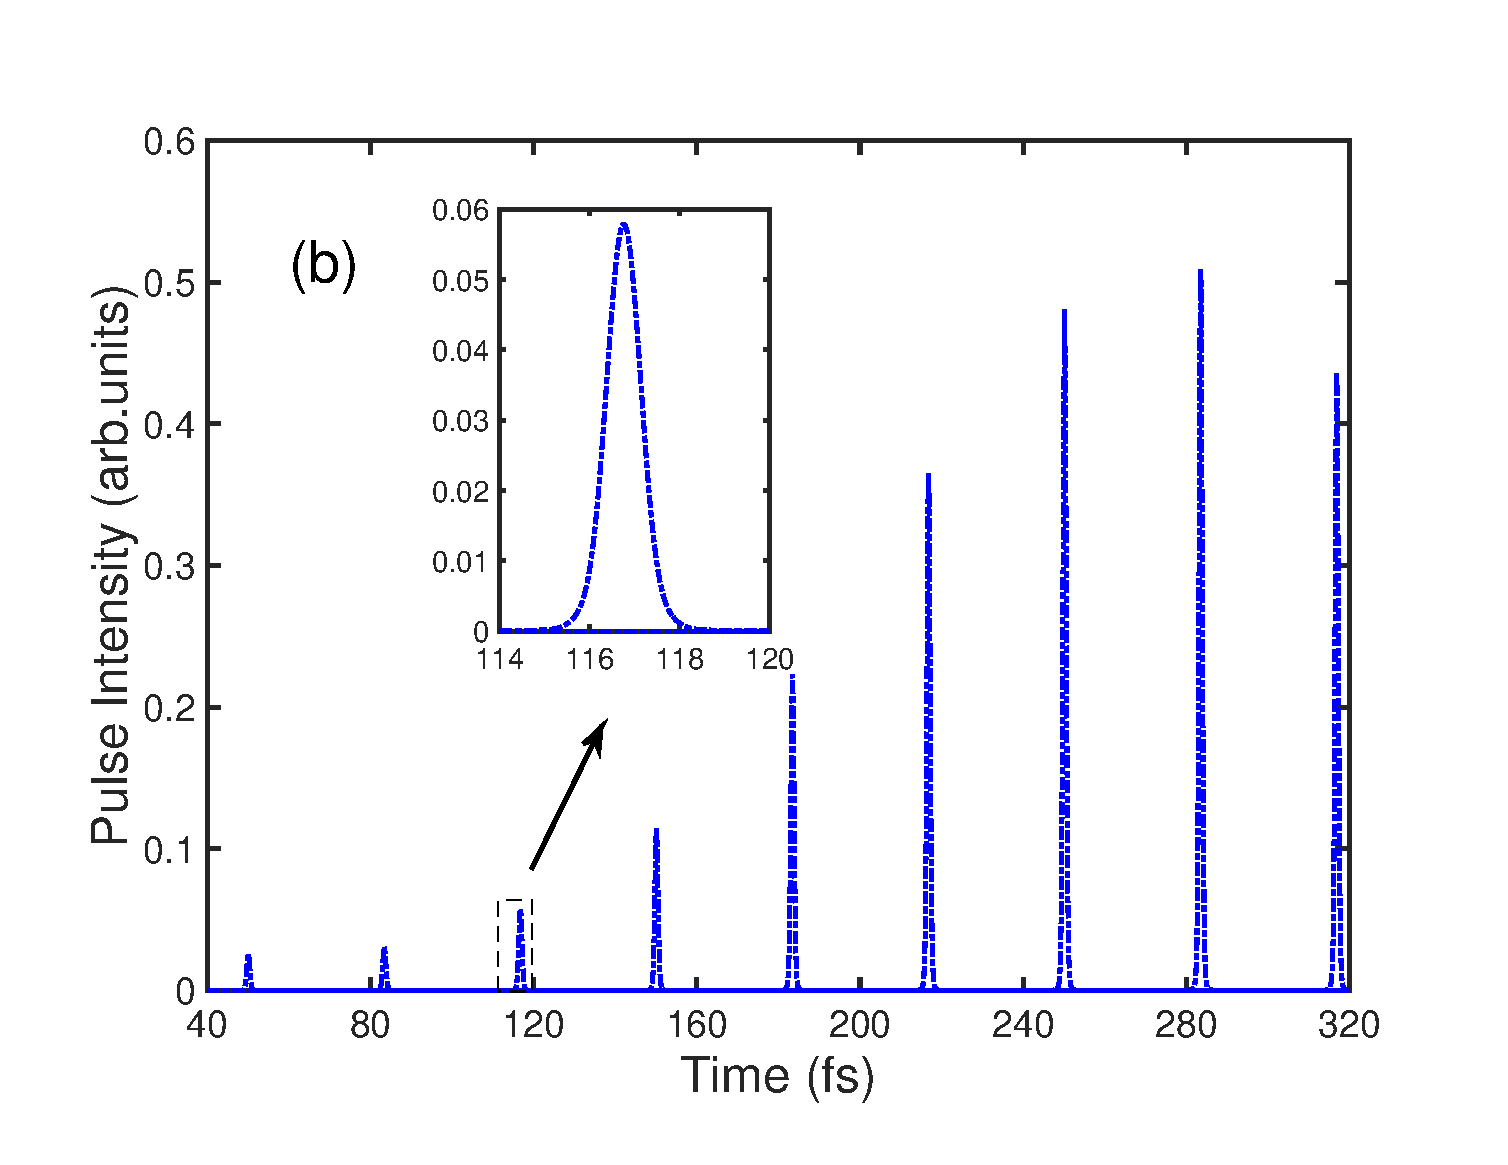
\includegraphics[width=0.4\textwidth]{fig7b.eps}
	}
	\caption{Isolated attosecond pulse from synthesizing the harmonics in the cutoff region of the spectrum which corresponds to Figs. \ref{fig6a} and \ref{fig6b}, respectively.}
	\label{fig7}
\end{figure}

We can also see from Fig. \ref{fig7} and Table \ref{table1} that, the chirped frequency has no help with the IAP generation because of the selecting of cutoff region harmonics instead of plateau region harmonics. Furthermore, even though the propagation can increase the intensity of cutoff region harmonics, it has hardly increased the plateau harmonics (seen from Fig. \ref{fig6}). Therefore, if we want to generate an IAP, the propagation is helpful. Otherwise, the propagation is not needed, and the medium should be low-density or thin enough. 

\begin{table}[!htbp]
	\centering
	\caption{Statistics for the isolated attosecond pulse's peak intensity and FWHM for the two cases of with and without chirp.}
\begin{tabular}{cccccc}
	\hline 
	Propagation & \multicolumn{2}{c}{Laser pulse without chirp} &  & \multicolumn{2}{c}{Laser pulse with chirp}\tabularnewline
	\cline{2-3} \cline{5-6} 
	distance ($\mu m$) & Peak intensity (arb.units) & FWHM (as) &  & Peak intensity (arb.units) & FWHM (as)\tabularnewline
	\hline 
	10 & 0.32 & 325 && 0.03 & 950\tabularnewline
	20 & 0.25 & 325 && 0.03 & 950\tabularnewline
	30 & 0.19 & 300 && 0.06 & 980\tabularnewline
	40 & 0.14 & 300 && 0.11 & 950\tabularnewline
	50 & 0.13 & 300 && 0.22 & 950\tabularnewline
	60 & 0.23 & 300 && 0.36 & 980\tabularnewline
	70 & 0.46 & 300 && 0.48 & 950\tabularnewline
	80 & 0.48 & 300 && 0.51 & 950\tabularnewline
	90 & 0.09 & 300 && 0.44 & 950\tabularnewline
	\hline 
\end{tabular}
	\label{table1}

\end{table}

\section{Conclusions}
In this paper, we tried to combine the control of the matter and the control of the driven laser pulse to produce a high-order harmonic spectrum with a higher cutoff energy and strong coherence. It is shown that the existence of the permanent dipole moments can significantly extend the plateau of the harmonic spectrum. If the laser pulse is modulated by added chirped frequency, the up-down symmetry of the laser field will be dramatically changed. This kind of laser pulse can exactly enhance the coherence of the harmonics in a large range in the plateau of the high-order harmonic spectrum. Finally, an attosecond pulse train with only two individual peaks is generated by Fourier synthesis of the harmonics within the plateau region. If the propagation effect is considered, an isolated attosecond pulse with considerable intensity can be generated by synthesizing the harmonics in the spectrum cutoff region for a proper propagation distance.

\section*{Acknowledgments}
This work is supported by the National Natural Science Foundation of China (NNSF, Grant
No.11374318). C.L. appreciates the supports from the 100-Talents Project of Chinese Academy
of Sciences and Department of Human Resources and Social Security of China.

\end{document}

